\documentclass[11pt, a4paper]{article}
\usepackage[utf8]{inputenc}

\usepackage{listings}
\usepackage[framed,numbered,autolinebreaks,useliterate]{mcode}

\usepackage[margin=1in]{geometry}
\usepackage{graphicx}
\usepackage{amsmath}
\usepackage{amsfonts}
\usepackage{float}
\graphicspath{ {../images/} }
\setlength\parindent{0pt}


\newcommand{\p}{\partial}
\newcommand{\mth}[1]{
  \begin{align*}
    #1
  \end{align*}
}



\begin{document}

\begin{center}
  \Huge ECEN4532, DSP Laboratory \\
  \huge Rhythm and Tone \\
  \huge Lab 2\\
  
  \vspace{7in}
    \huge Jeffery Lim \\
    \huge Jeffery.Lim@colorado.edu\\~\\~\\
\end{center}
\pagebreak


\tableofcontents

\pagebreak

\section{Introduction}

For this lab, the rhythm and tone were extracted from the song. First, a similarity matrix is constructed by comparing each frame with the frames next to it. After, using the similarity matrix, rhythm can be extracted using three different methods. Finally, tones can be found by taking the MFCC matrix found from the previous lab and generate a normalized pitch class profile. 

\section{Similarity}

\lstinputlisting[language=Matlab]{../similarity.m}

\begin{figure}[H]
    \centering
    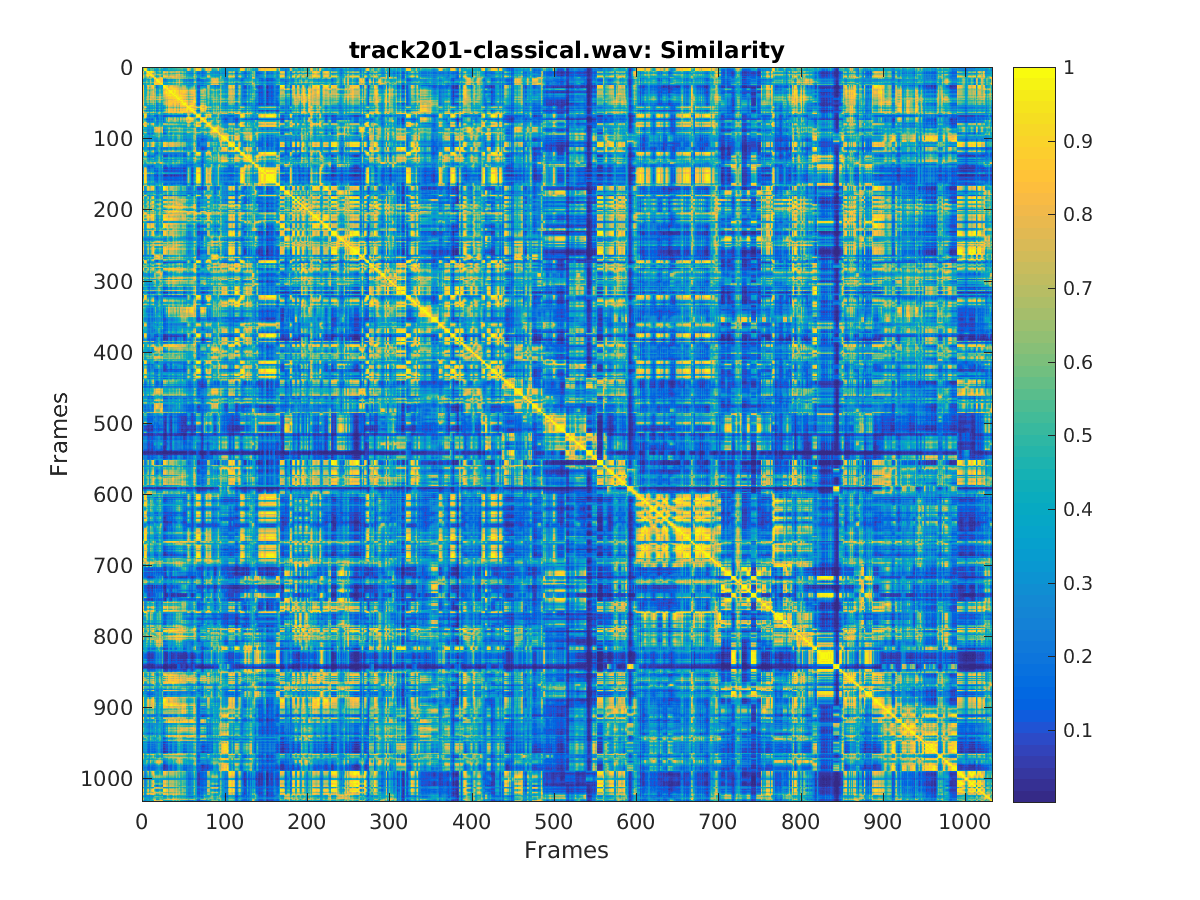
\includegraphics[width=.8\textwidth]{track201-classical-similarity.png}
    \caption{track201-classical}
\end{figure}

There is very little similarity in this song. There is a small section that is similar, but overall, the song's shape is not the same.

\begin{figure}[H]
    \centering
    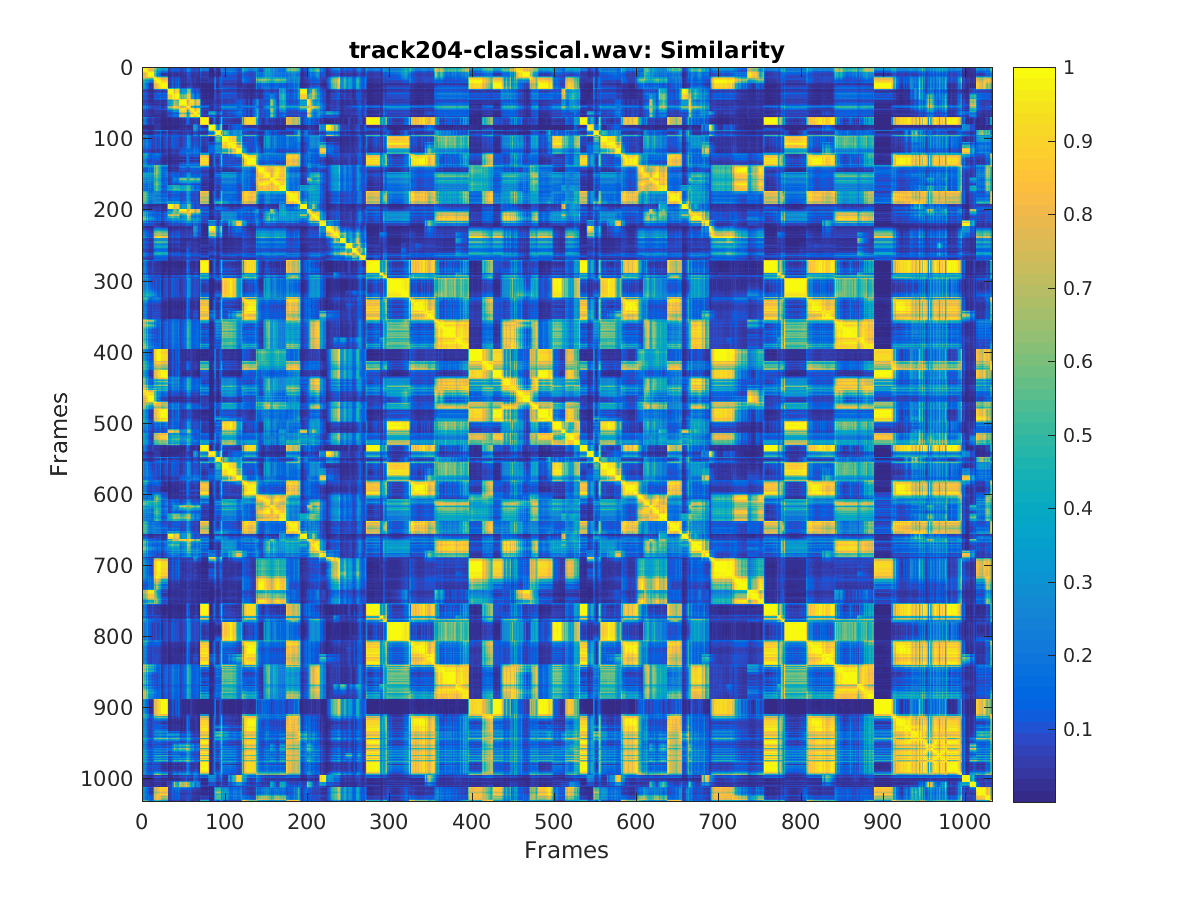
\includegraphics[width=.8\textwidth]{track204-classical-similarity.png}
    \caption{track204-classical}
\end{figure}

This piano piece may have a lot of similarity because there are notes that may be played multiple times. This would result in the similarity matrix to have a magnitude of 1 when the same notes are being played, a common occurrence in some classical music. 	


\begin{figure}[H]
    \centering
    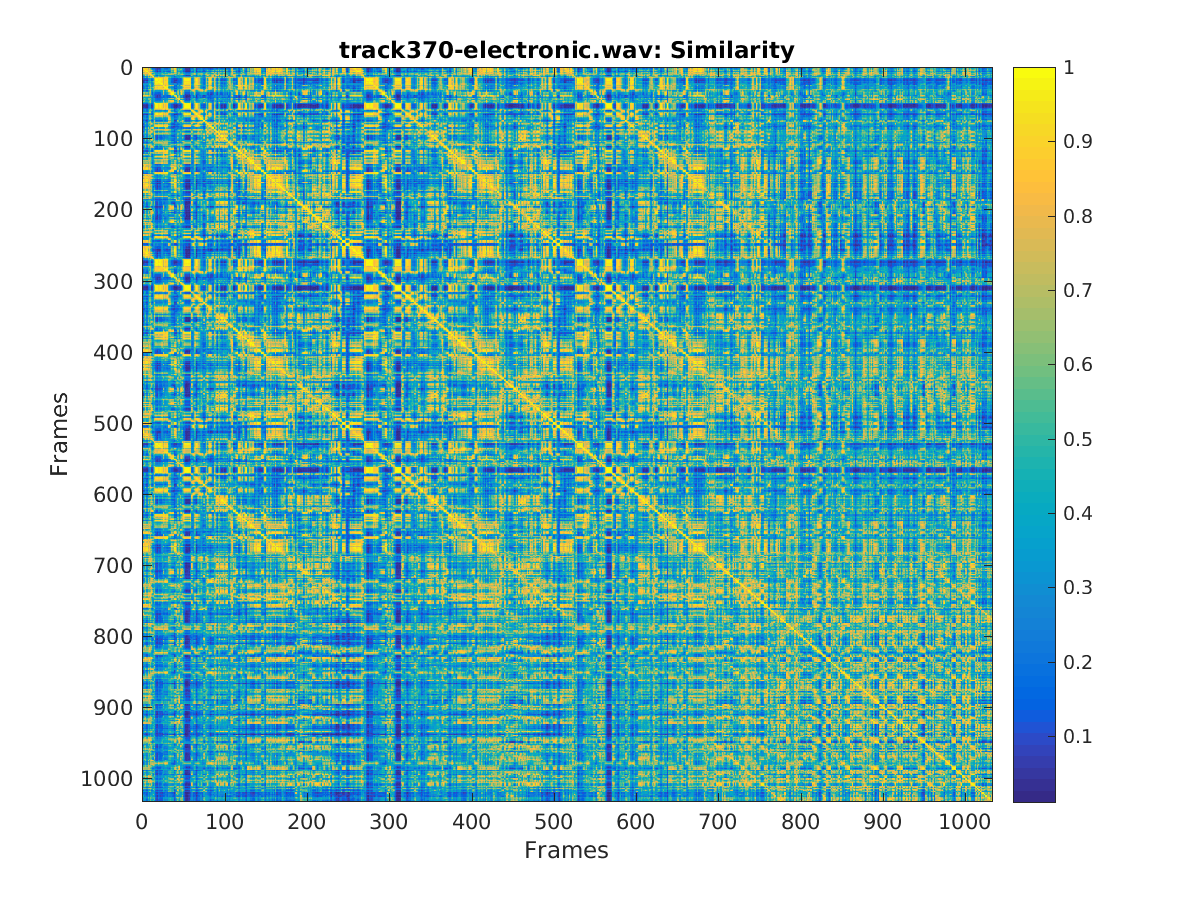
\includegraphics[width=.8\textwidth]{track370-electronic-similarity.png}
    \caption{track370-electronic}
\end{figure}

The beginning part of the song has some similarites, and there is a very obvious shift of the song's composition at around 700 frames.

\begin{figure}[H]
    \centering
    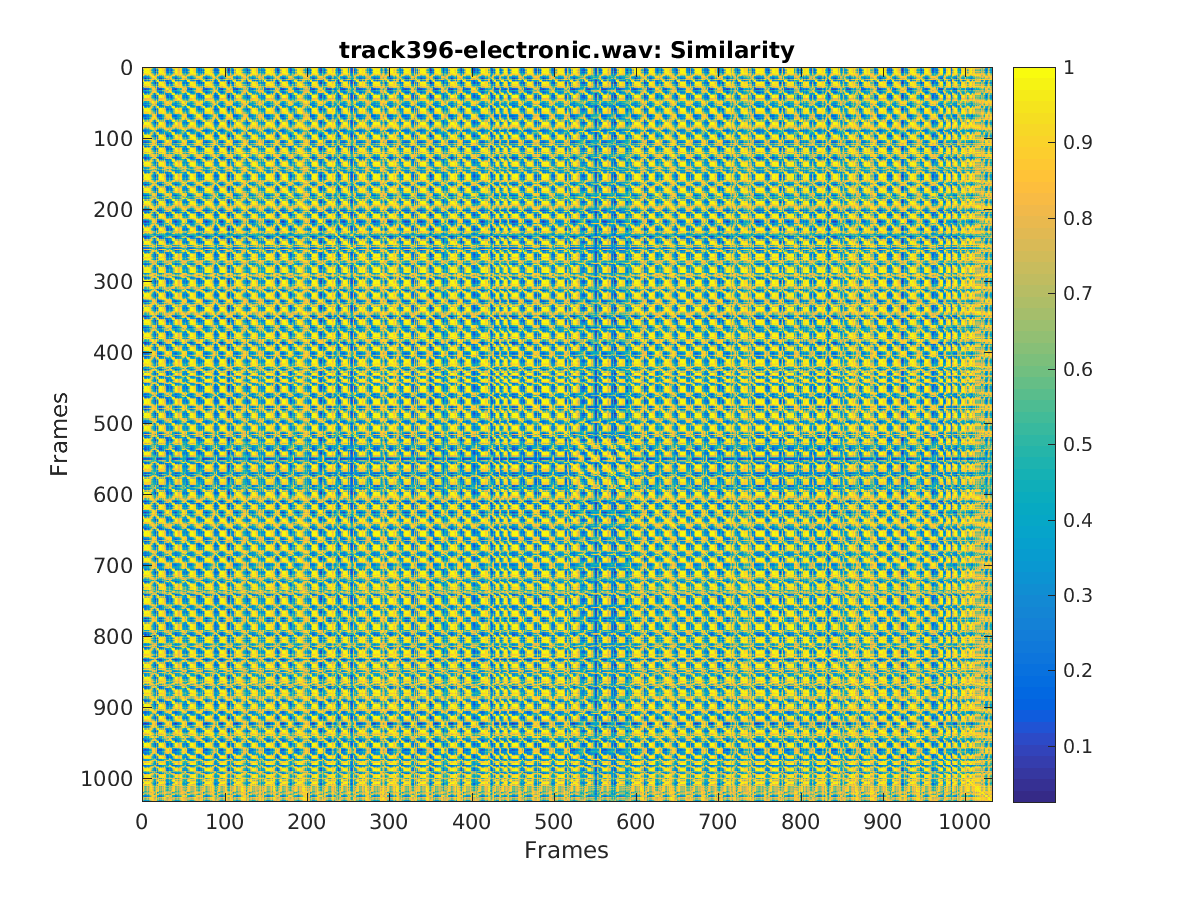
\includegraphics[width=.8\textwidth]{track396-electronic-similarity.png}
    \caption{track396-electronic}
\end{figure}

The underlying beat in this song is clearly seen throughout the entire image, and demonstrates that there is very similar notes being played. As expected for an electronic song, the repetitive beats and sounds may cause the similarity matrix to show that many of the frames are similar to each other.

\begin{figure}[H]
    \centering
    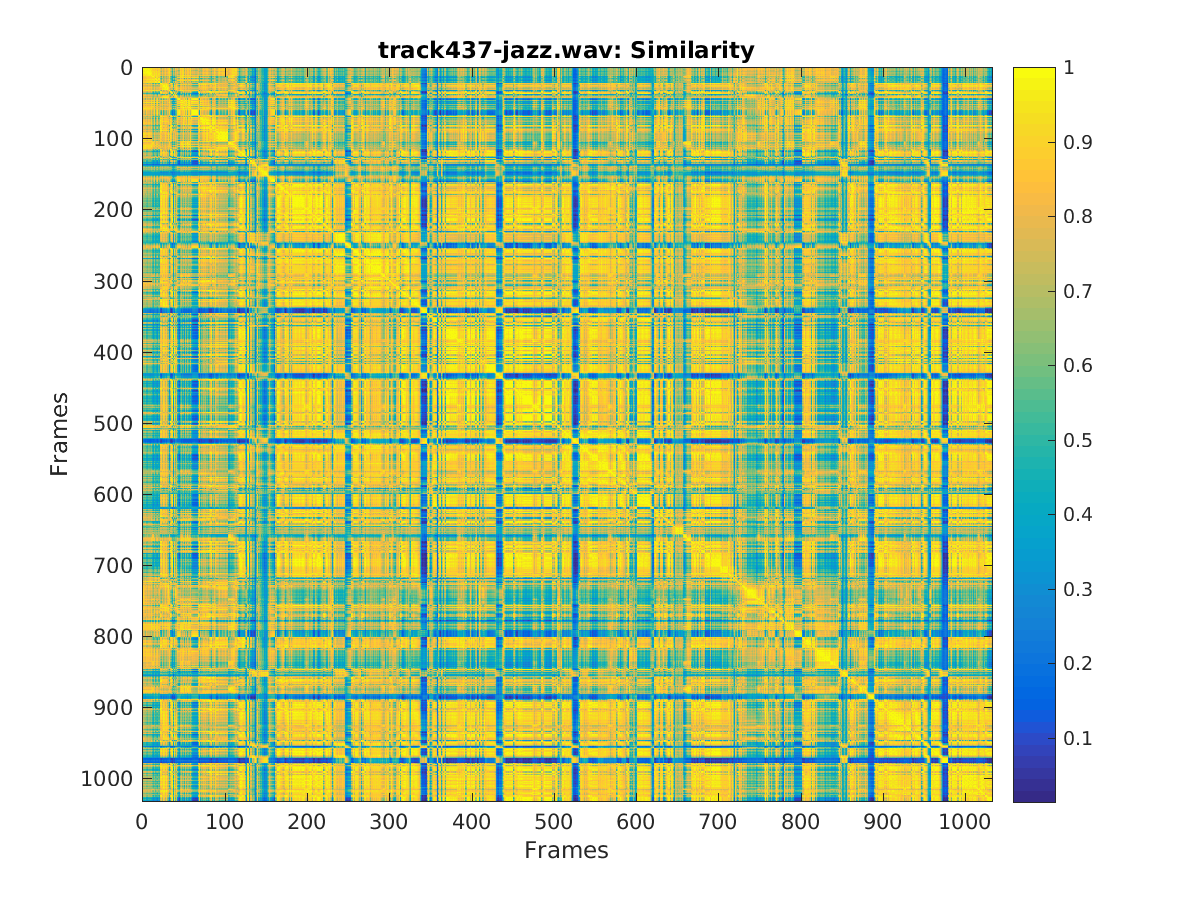
\includegraphics[width=.8\textwidth]{track437-jazz-similarity.png}
    \caption{track437-jazz}
\end{figure}

The jazz track has some similarities at many frames, similar to the electronic tracks. This makes it seem that the similarity matrix does not necessarily discern different genres, but gives information on the song's composition.

\begin{figure}[H]
    \centering
    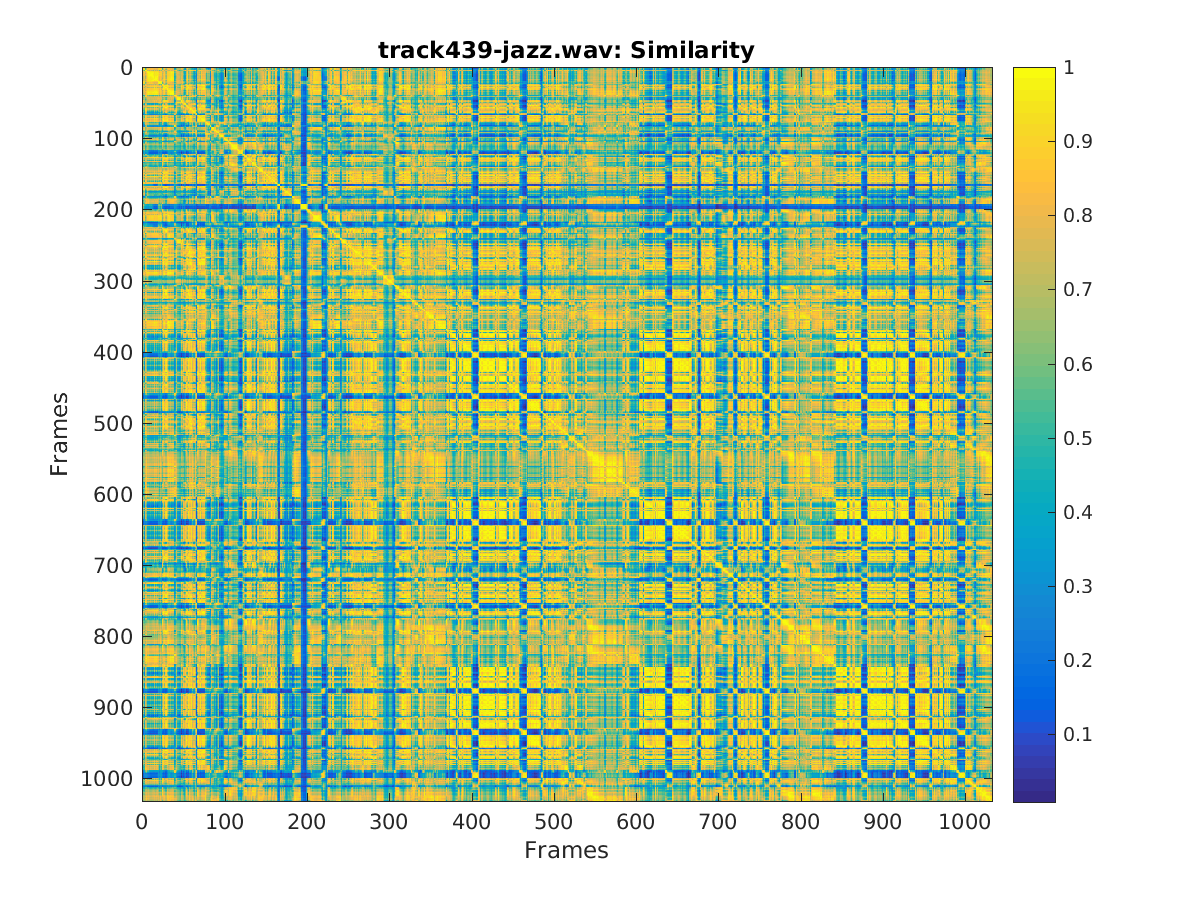
\includegraphics[width=.8\textwidth]{track439-jazz-similarity.png}
    \caption{track437-jazz}
\end{figure}

It is interesting to note that this jazz track is similar to the previous one, which may reveal an underlying pattern between all jazz genres. 

\begin{figure}[H]
    \centering
    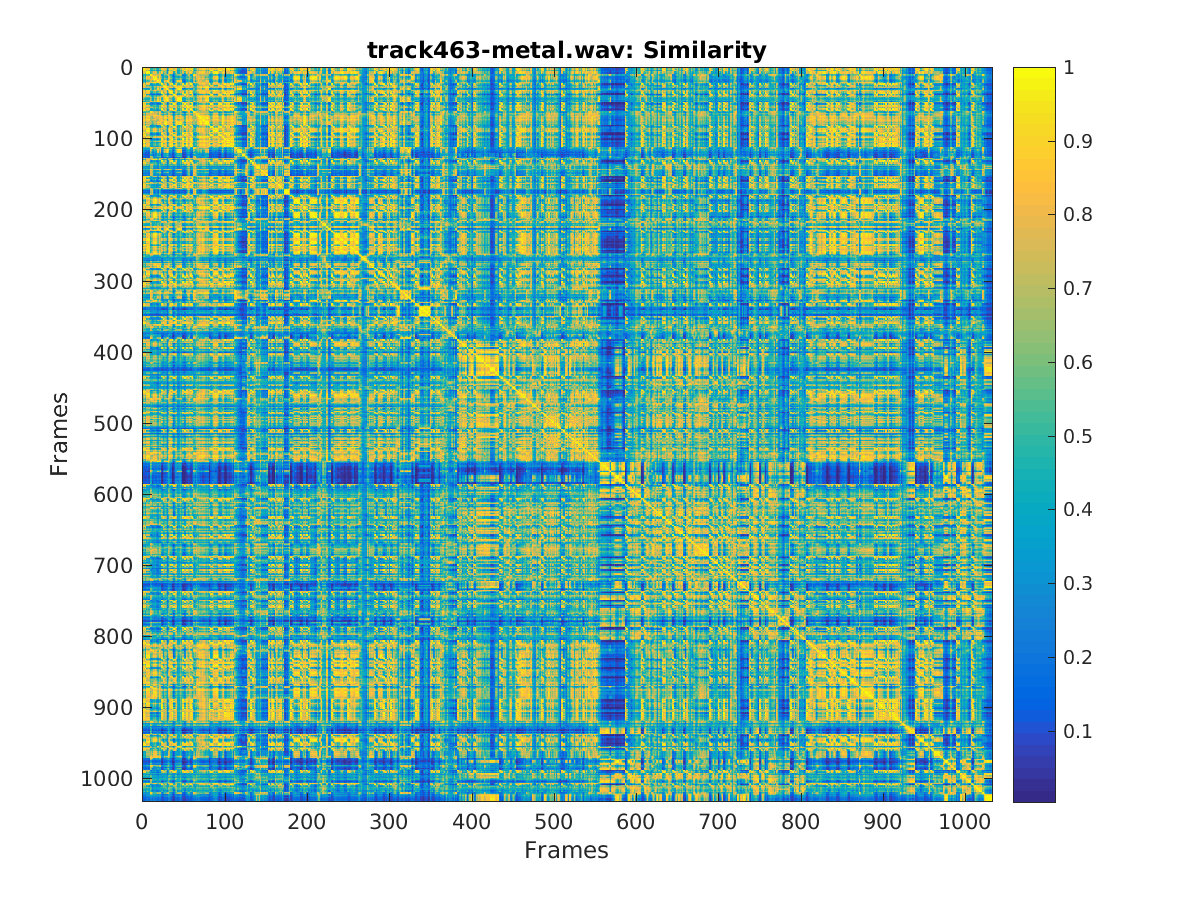
\includegraphics[width=.8\textwidth]{track463-metal-similarity.png}
    \caption{track463-metal}
\end{figure} 

There are some similarities between frames, but not much. It is hard to discern useful information from this matrix than others. 

\begin{figure}[H]
    \centering
    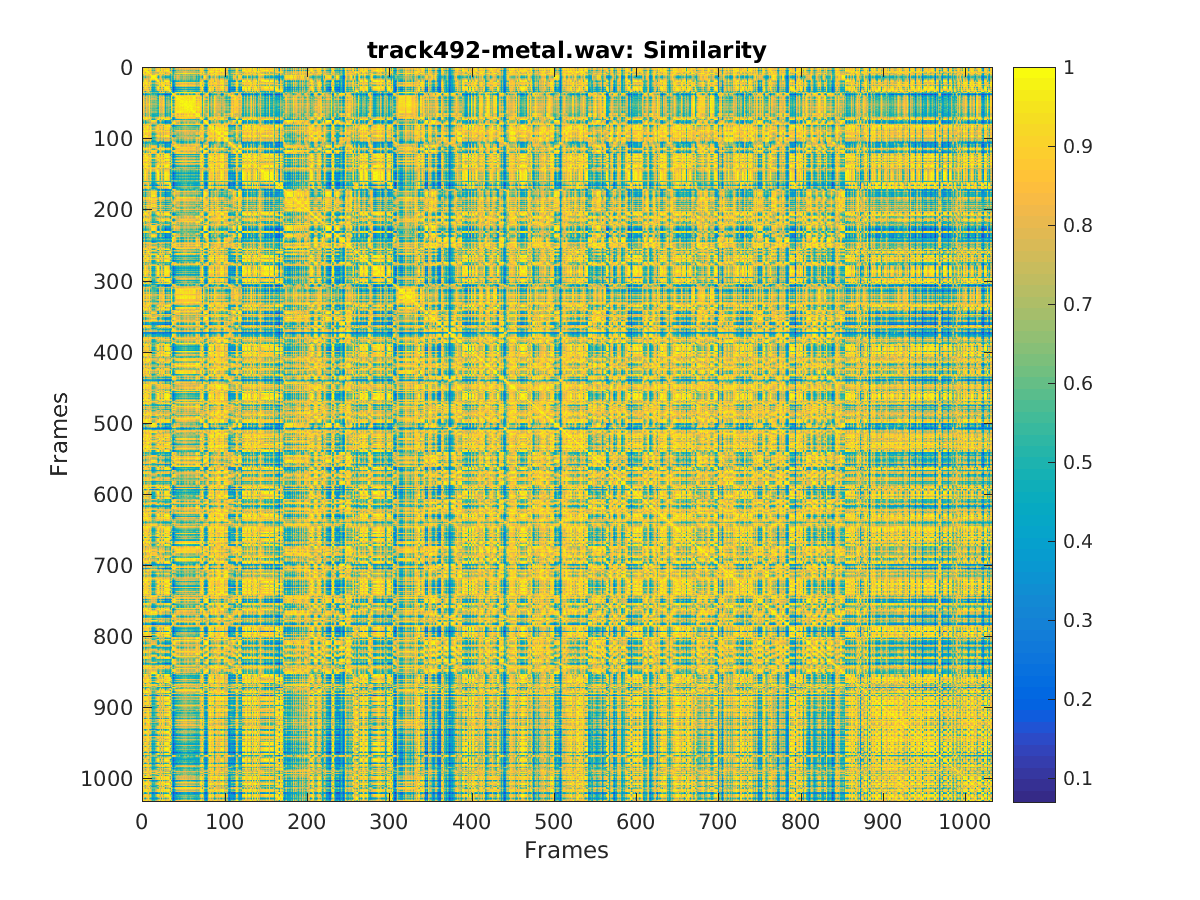
\includegraphics[width=.8\textwidth]{track492-metal-similarity.png}
    \caption{track492-metal}
\end{figure}

Very different from the previous metal song, but may share some confusion between electronic and this track. This simply means that a lot of the frames are similar to each other, but this is also a characteristic of other genres. 

\begin{figure}[H]
    \centering
    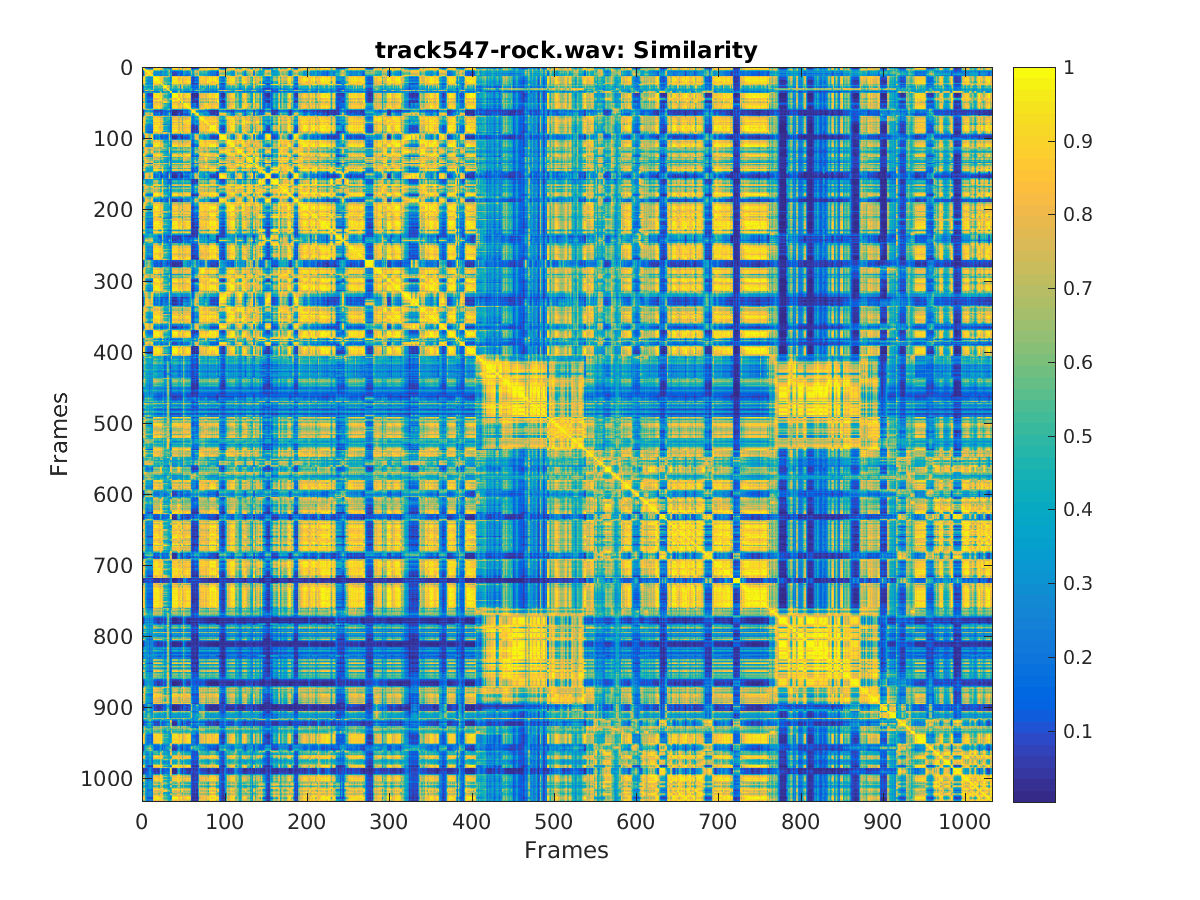
\includegraphics[width=.8\textwidth]{track547-rock-similarity.png}
    \caption{track547-rock}
\end{figure}

Shares a lot of similarities with the jazz track, which further confirms the difficulties of using this method to determine genre. 

\begin{figure}[H]
    \centering
    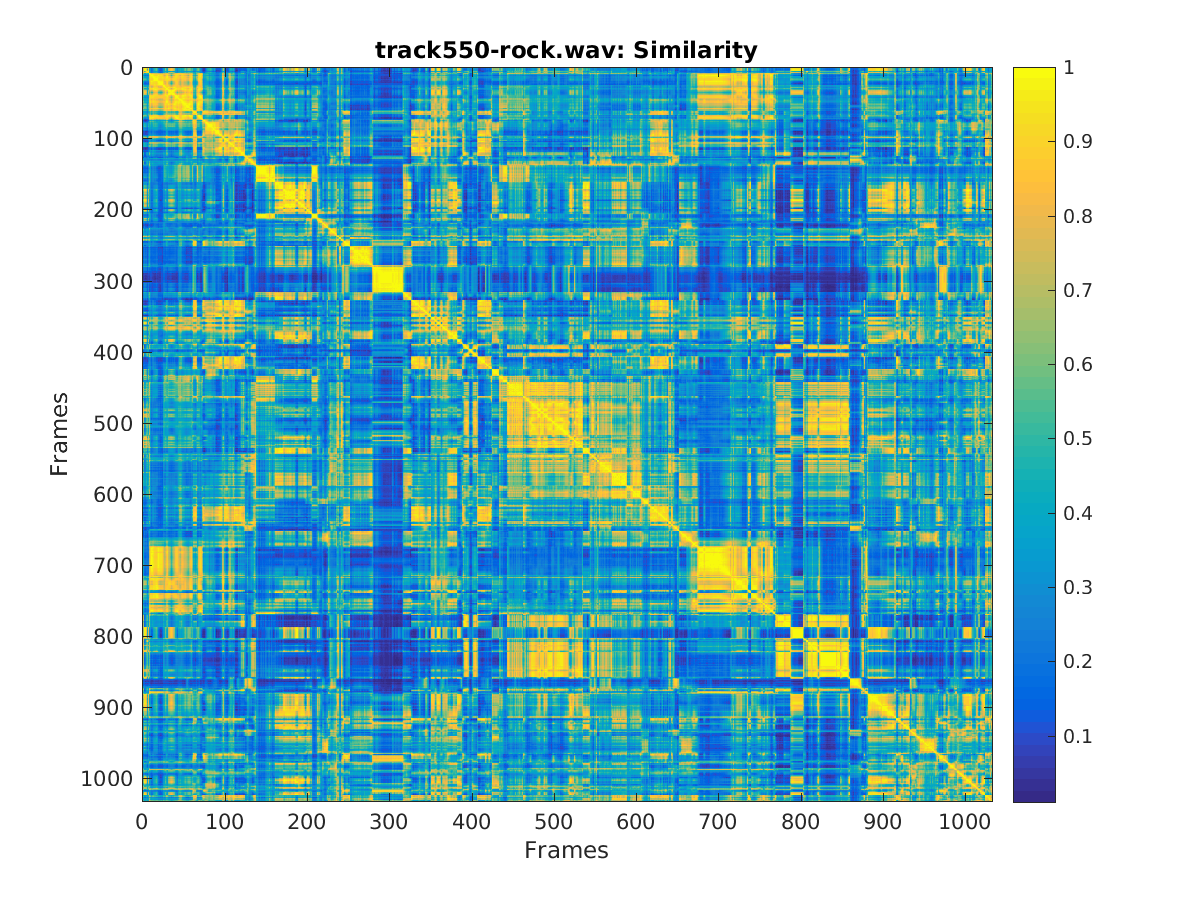
\includegraphics[width=.8\textwidth]{track550-rock-similarity.png}
    \caption{track550-rock}
\end{figure}

This track is very different from the previous rock and has no definite features. 


\begin{figure}[H]
    \centering
    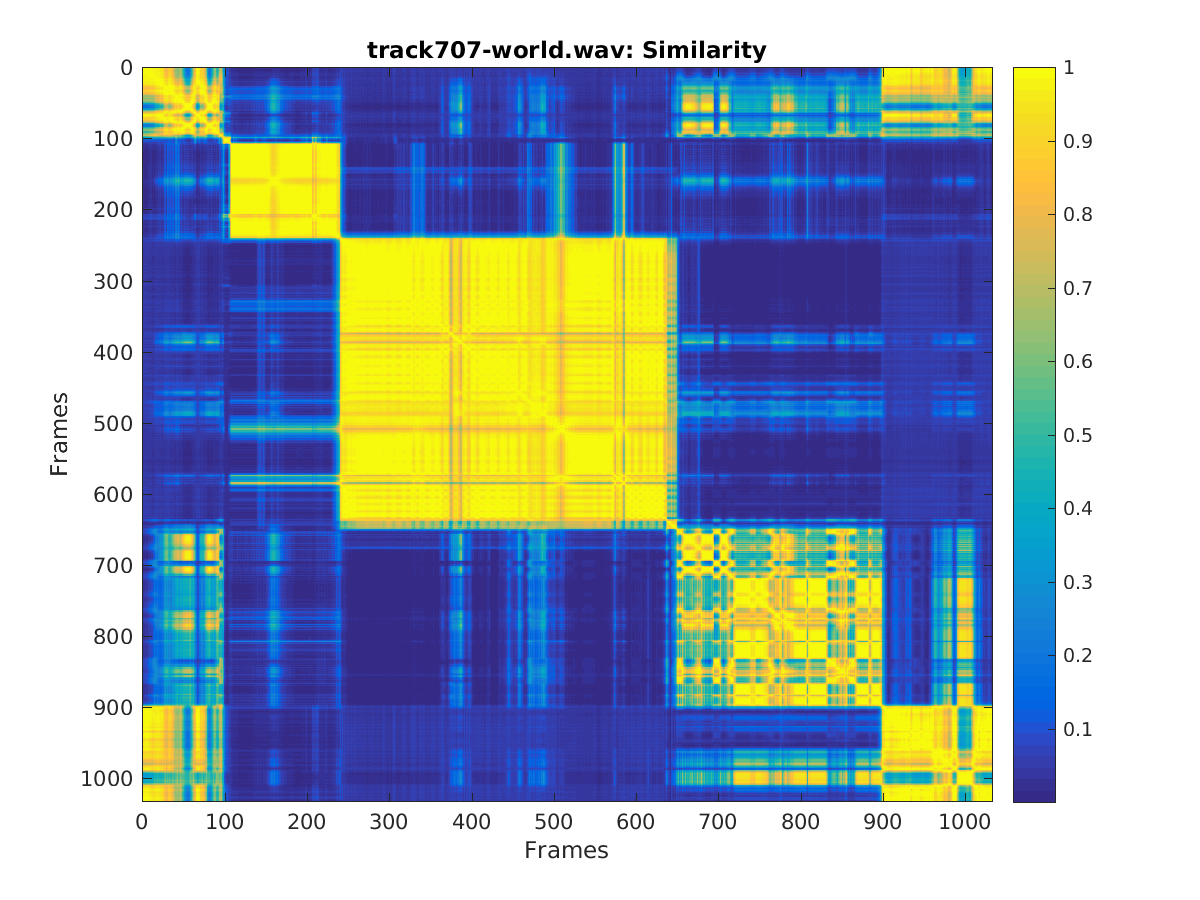
\includegraphics[width=.8\textwidth]{track707-world-similarity.png}
    \caption{track707-world}
\end{figure}

The pure tones being played at certain frames are very obvious to be similar and have the big chunk of similarities. It is easy to tell with this matrix that a single note is being played because of how solid the section of the similarity matrix is. 


\begin{figure}[H]
    \centering
    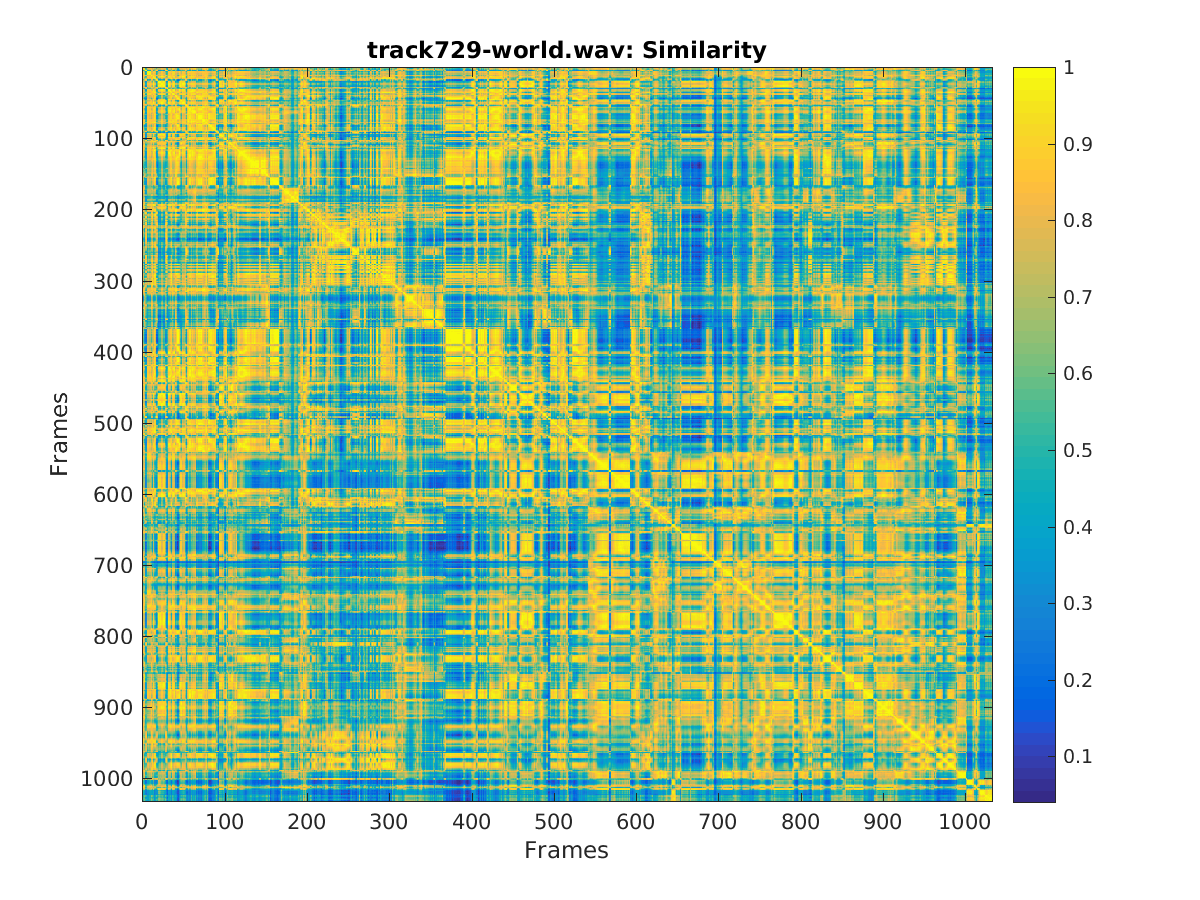
\includegraphics[width=.8\textwidth]{track729-world-similarity.png}
    \caption{track729-world}
\end{figure}

This has similarites to the jazz and the rock tracks

\subsection{Conclusion: Similarity}

The similarity matrices demonstrate beats or rhythms that can be found, however, there are underlying issues with being able to differentiate from the genres. 
	

\section{Rhythm}

For rhythm, three different rhythm detectors are designed and each will be compared. In each of the images, the top image is the first estimate of rhythm, the middle image is the second better estimate of rhythm, and the last image is the dynamic rhythmic variations over time. 

\lstinputlisting[language=Matlab]{../rhythmB.m}


\lstinputlisting[language=Matlab]{../rhythmAR.m}


\lstinputlisting[language=Matlab]{../dynamicRhythmAR.m}


\begin{figure}[H]
    \centering
    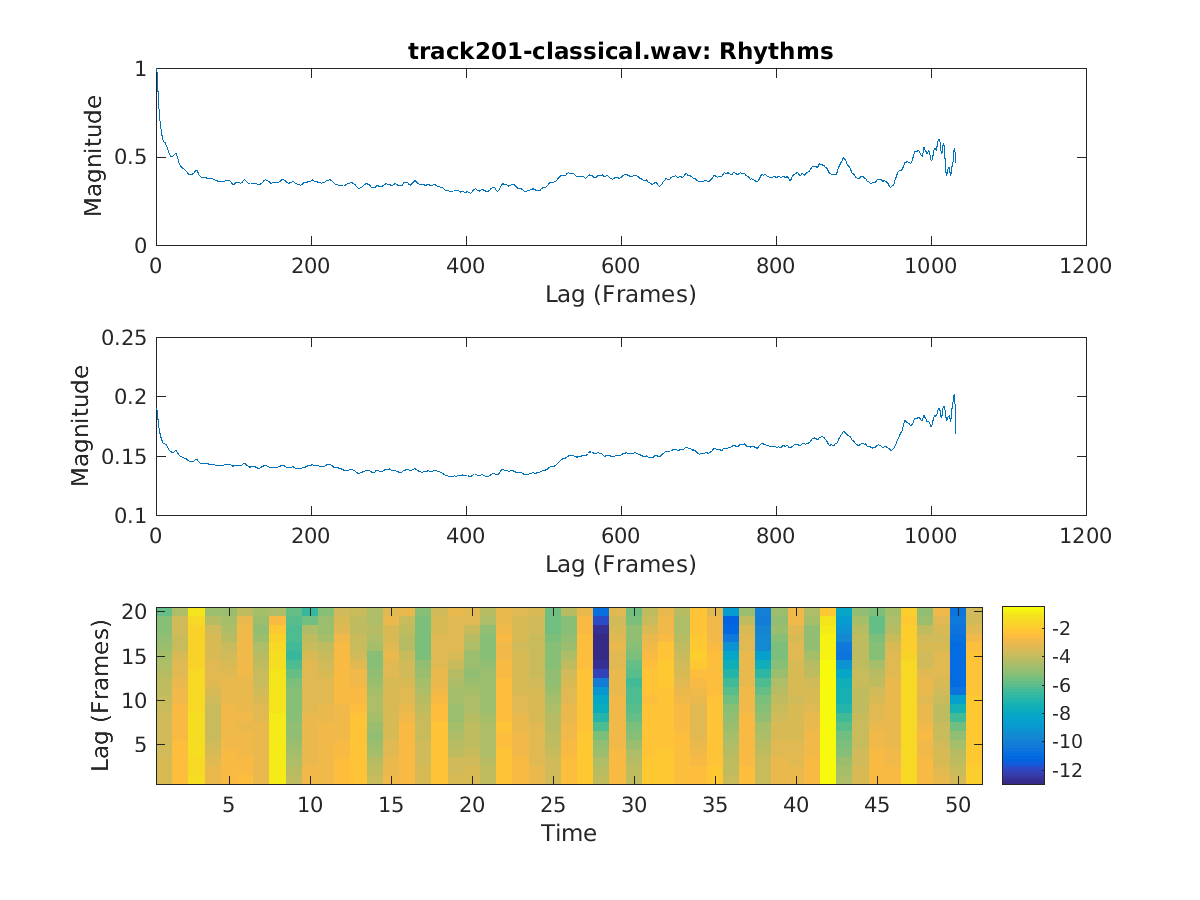
\includegraphics[width=.8\textwidth]{track201-classical-Rhythm.png}
    \caption{track201-classical}
\end{figure}

The first rhythm and second rhythm are very similar, with the only difference being the magnitudes. As evident by the shape of the graph, there is not much of a rhythm presence. \\

For the rhythmic variations, its evident that there is not much variations throughout the song, however, at times 3 and 7, there is a flipped repeat of it later at 42 and 47, however, this is not necessarily a rhythm. 

\begin{figure}[H]
    \centering
    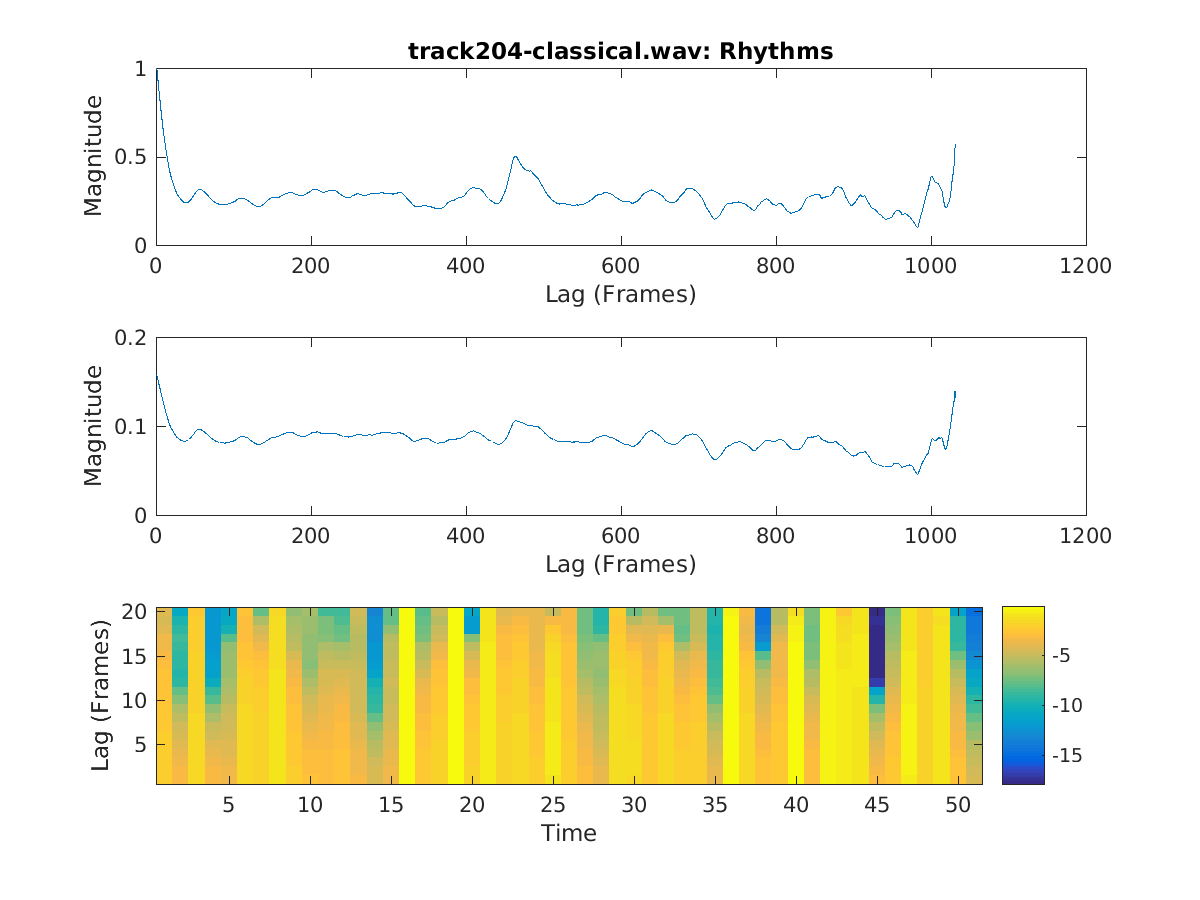
\includegraphics[width=.8\textwidth]{track204-classical-Rhythm.png}
    \caption{track204-classical}
\end{figure}

Again, like the previous track, the first and second rhythm plots are very similar, with a difference in the magnitudes. There is a presense of some rhythm, but it is not very consistent and it is hard to tell if there a very defined rhythm in the song. \\

For the rhythmic variations, there is not that many variations through the song at each time frame. Through those frames, there is actually no significant differences between them. 


\begin{figure}[H]
    \centering
    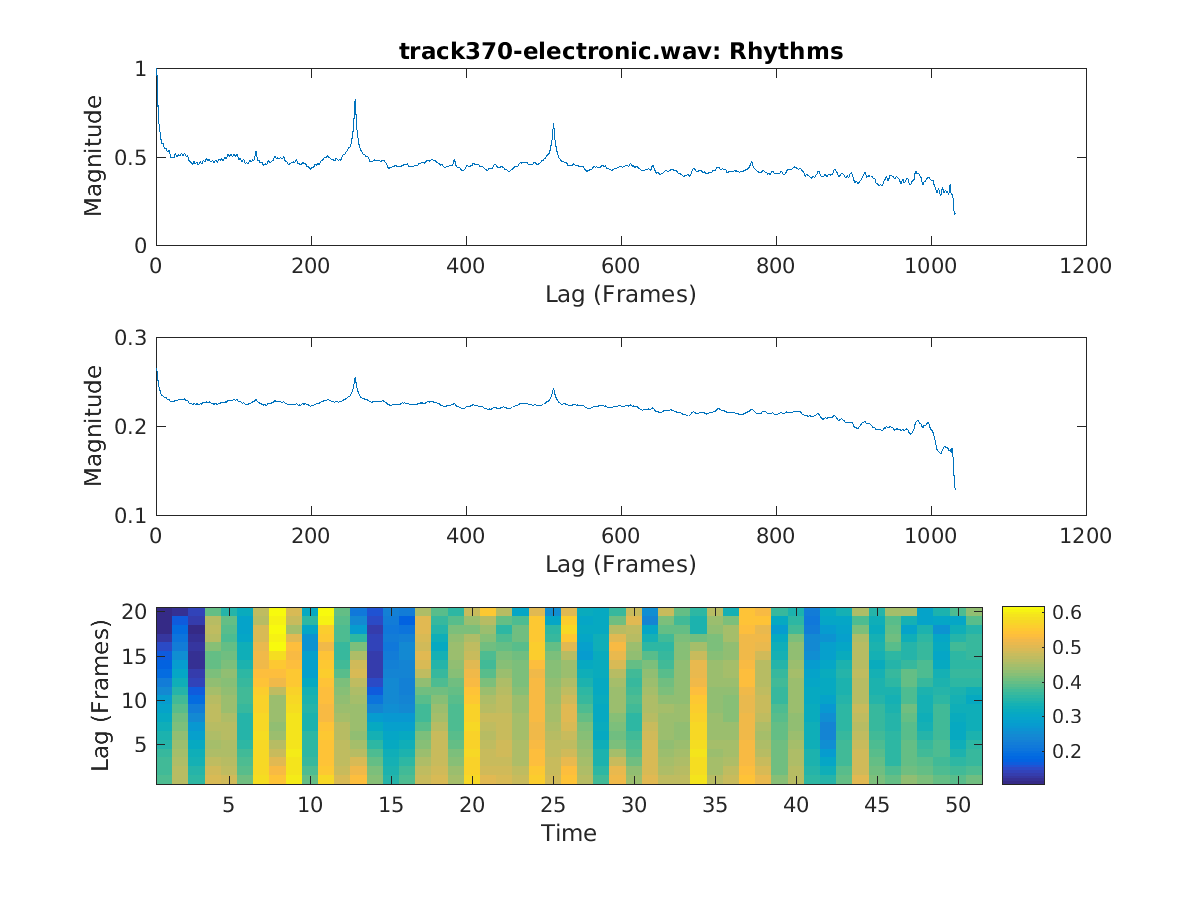
\includegraphics[width=.8\textwidth]{track370-electronic-Rhythm.png}
    \caption{track370-electronic}
\end{figure}

The electronic track should expect some rhythm component to be seen, and there is two significant spikes in both the first and second rhythm. \\

For the rhythmic variations, at each time, the frames seem to be changing significantly from time to time, and at around 16 or 17 seconds, there is an evident repeat at the same time as at around 30 seconds. This is clear evidence of some sort of pattern occurring, but not a very strong one. 


\begin{figure}[H]
    \centering
    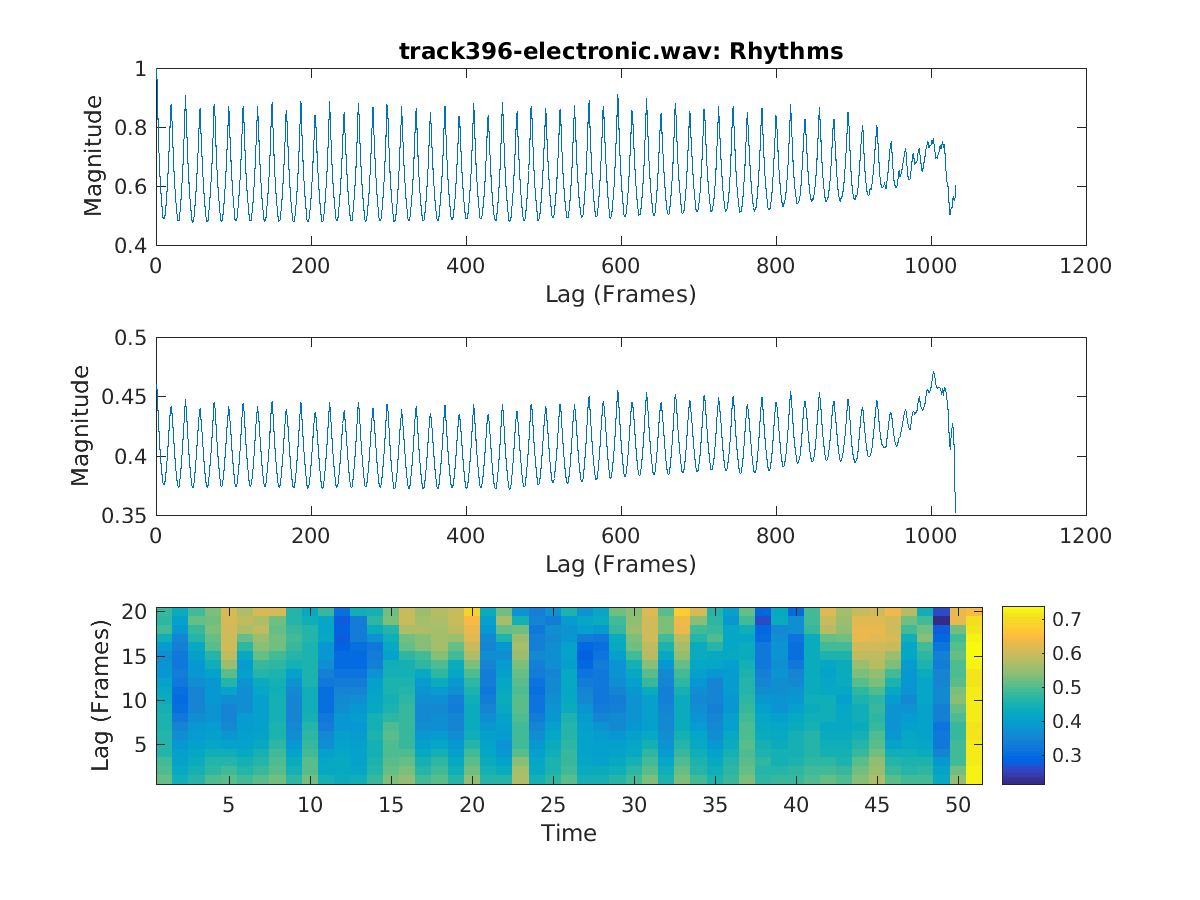
\includegraphics[width=.8\textwidth]{track396-electronic-Rhythm.png}
    \caption{track396-electronic}
\end{figure}

This track is very evident in its rhythm. There is a strong rhythm outlined in both plots. This rhythm is occur consistently throughout most of the frames in this track. \\

For the rhythmic variations, there is a clear repeat through the song of variations repeating over and over. \\

\begin{figure}[H]
    \centering
    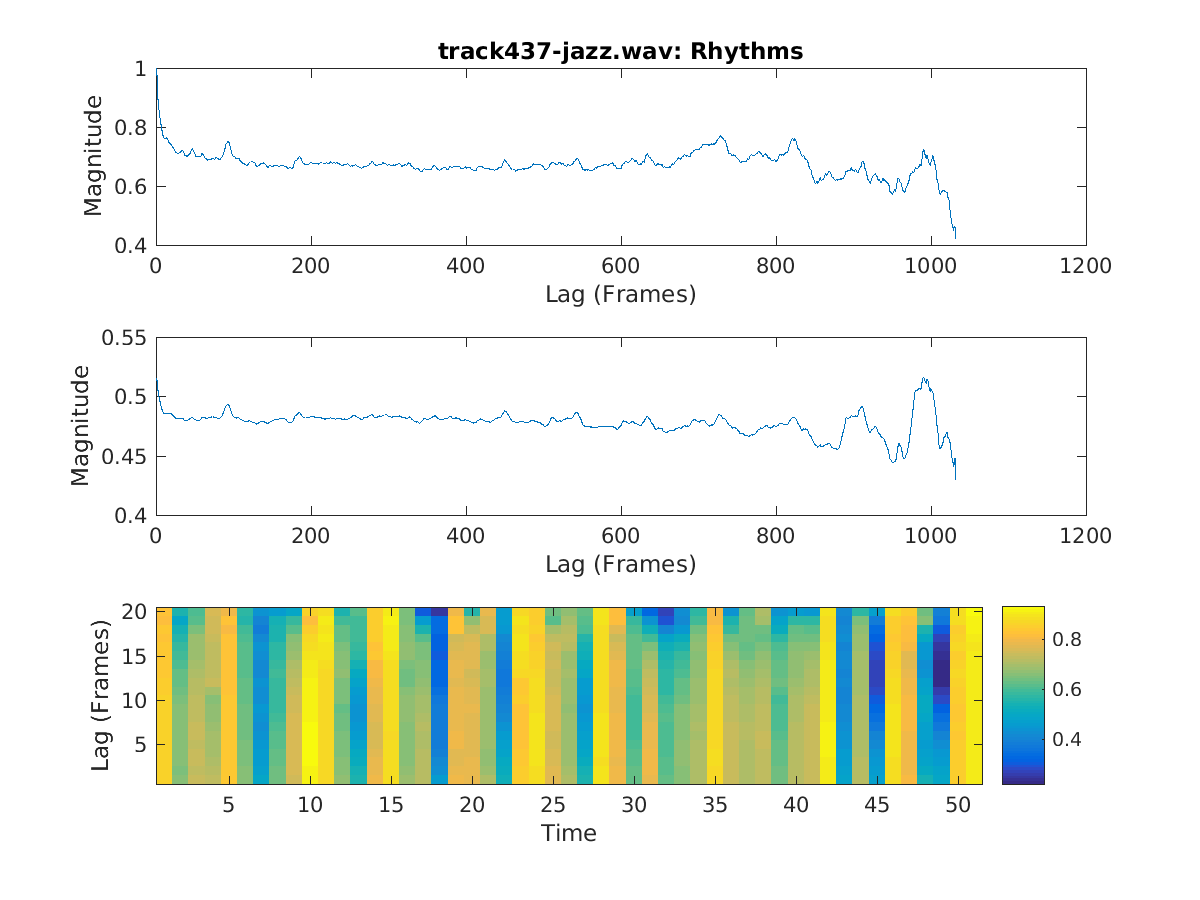
\includegraphics[width=.8\textwidth]{track437-jazz-Rhythm.png}
    \caption{track437-jazz}
\end{figure}

There are some rhythmic patterns, however, there is nothing that is strongly rhythmic because there are no repeating spikes in the magnitudes of either the first or second rhythm plots. \\

For the rhythmic variations, most of the time, the frames are all of the same color, and there are no repeating patterns at future times, and thus, it can be said there is very little rhythmic variations in the song. 

\begin{figure}[H]
    \centering
    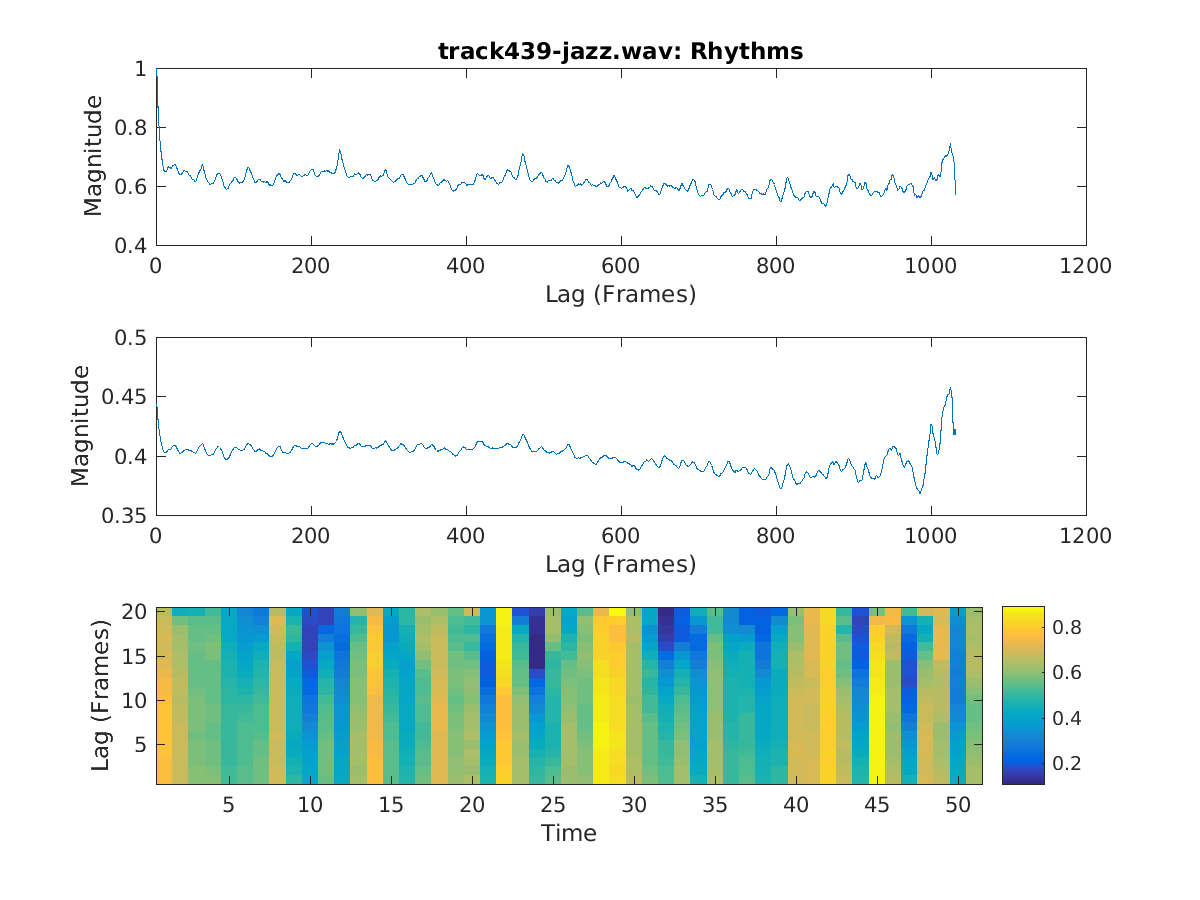
\includegraphics[width=.8\textwidth]{track439-jazz-Rhythm.png}
    \caption{track437-jazz}
\end{figure}

For the second jazz track, there are evidence of some rhythm patterns, however, there are strong rhythm patterns as evident by the lack of repeating spikes in either the first or second rhythm plot. \\

For the rhytmic variations, there are slight rhythm shifts throughout the song, however, like the second electronic tracks, there is no underly pattern that can picked out, and most of the variations are due to smaller frames being similar. 


\begin{figure}[H]
    \centering
    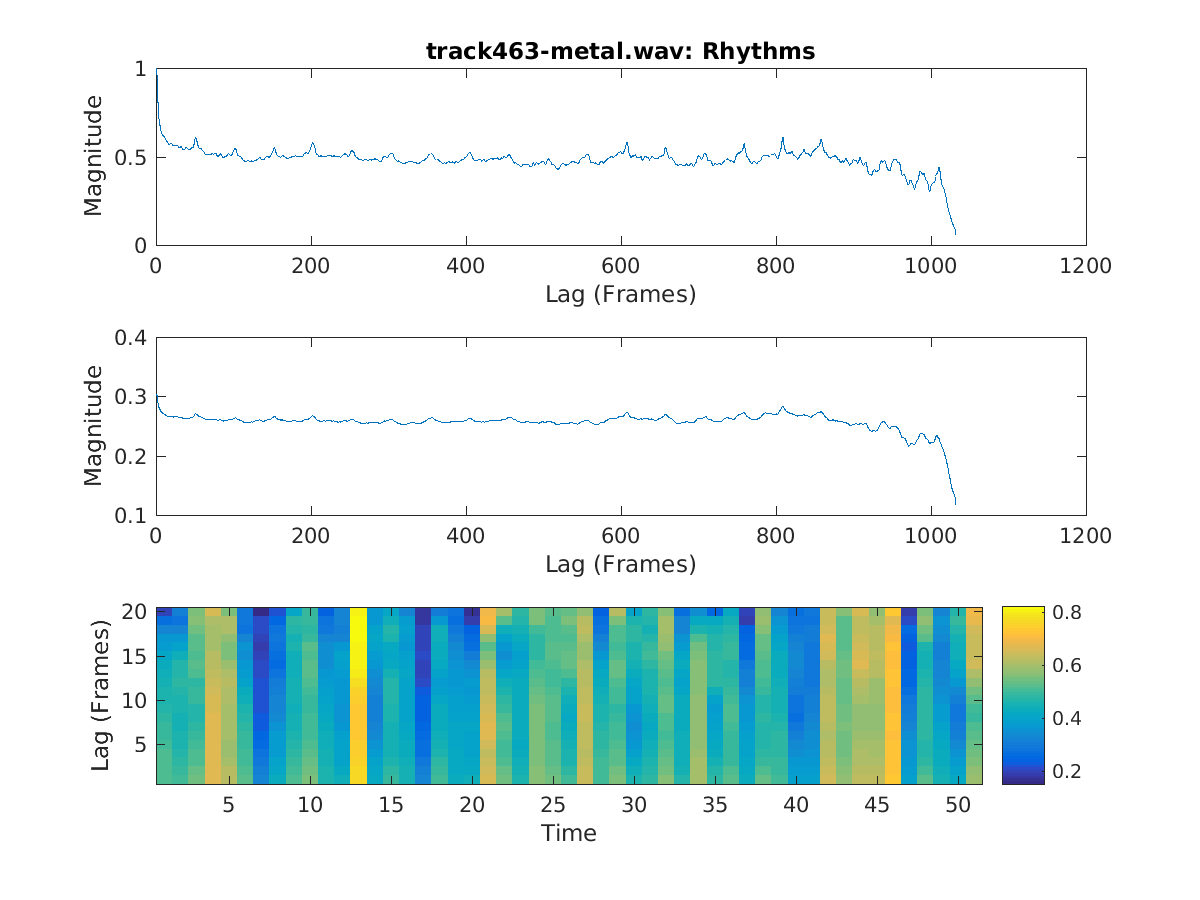
\includegraphics[width=.8\textwidth]{track463-metal-Rhythm.png}
    \caption{track463-metal}
\end{figure} 

There is evidence of a rhythmic pattern. It is hard to say whether it is strong because of the amplitudes are not as large in magnitude, but are repetitive. In the second plot, it seems that there is no real evidence of a strong rhythm pattern because the magnitudes of the spikes are not as large. This may mean, even though there is evidence of a pattern, it is not very strong or cannot be heard very well. \\

The rhythmic variations demonstrates that there are some changes between the frames at each time frame, but again, it is very weak and does not show a lot of variation. 

\begin{figure}[H]
    \centering
    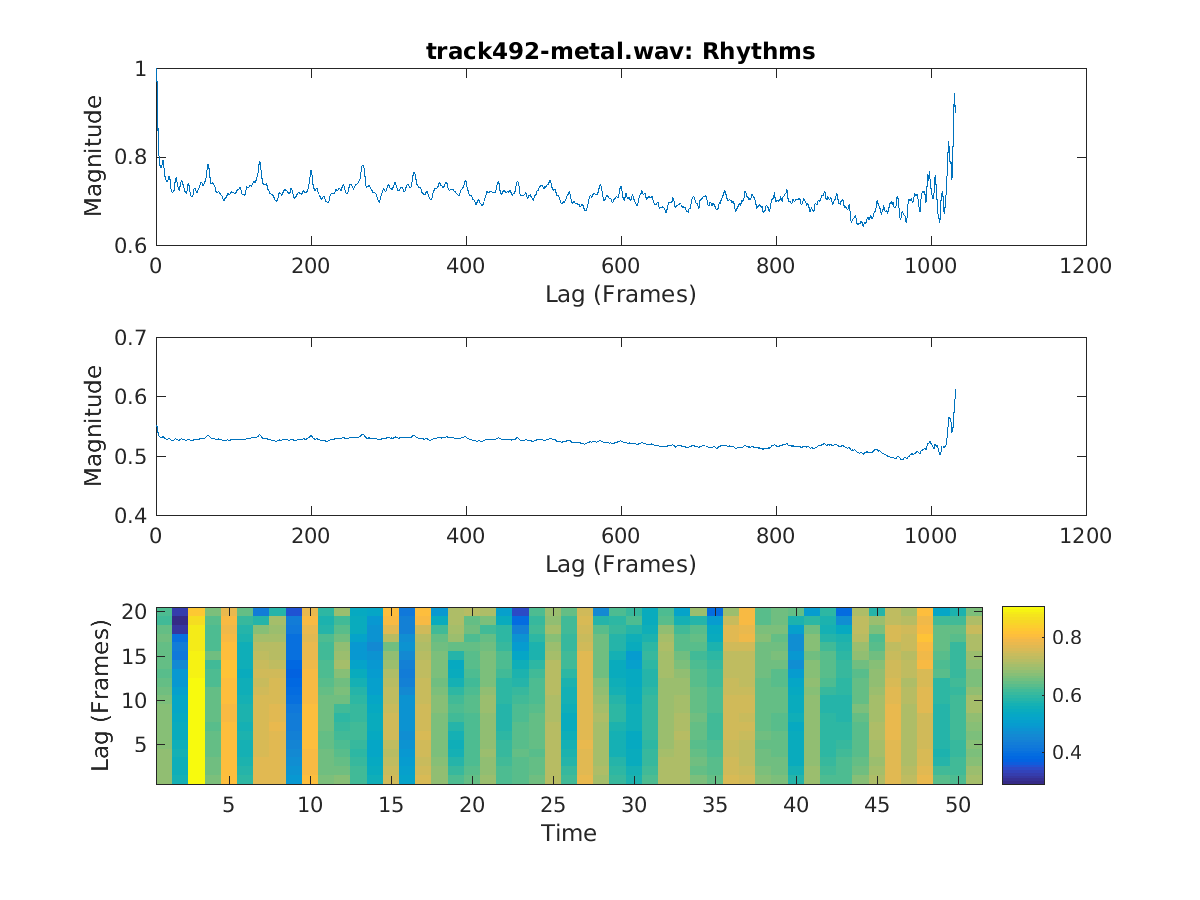
\includegraphics[width=.8\textwidth]{track492-metal-Rhythm.png}
    \caption{track492-metal}
\end{figure}

This metal track demonstrates strong pattern, as evident in the first rhythm plot. There is a consistent spike in the first hundred frames, which shares the mentality of the similarity matrix. When looking at the second rhythm plot, however, there is a flat line with very little changes in the magnitude. This sudden difference may demonstrate that the song is extremely noisy and thus, causing problems to be able to detect for the second rhythm plot. \\

For the rhythmic variations, there is evidence of some rhythm pattern occurring, but it is only for the first 30 seconds, and is also filled with other non rhythmic patterns that may seep into the song with the other instruments that are playing. 

\begin{figure}[H]
    \centering
    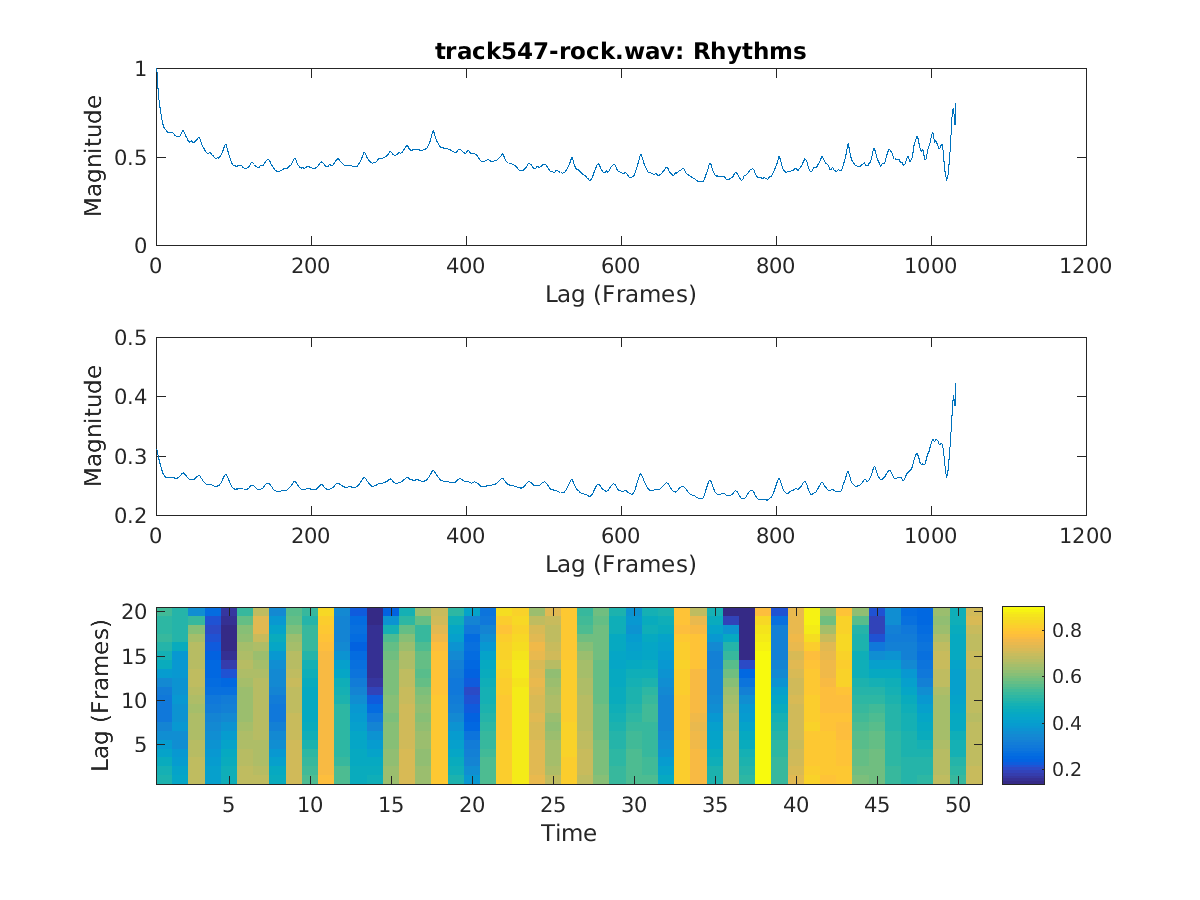
\includegraphics[width=.8\textwidth]{track547-rock-Rhythm.png}
    \caption{track547-rock}
\end{figure}

This rock track has a lot of spikes in the first rhythm, which indicates a rhythm pattern. The second plot also demonstrates a similar plot as well. \\

For the variation, there are slight changes, but no large overlying rhythmic patterns.  

\begin{figure}[H]
    \centering
    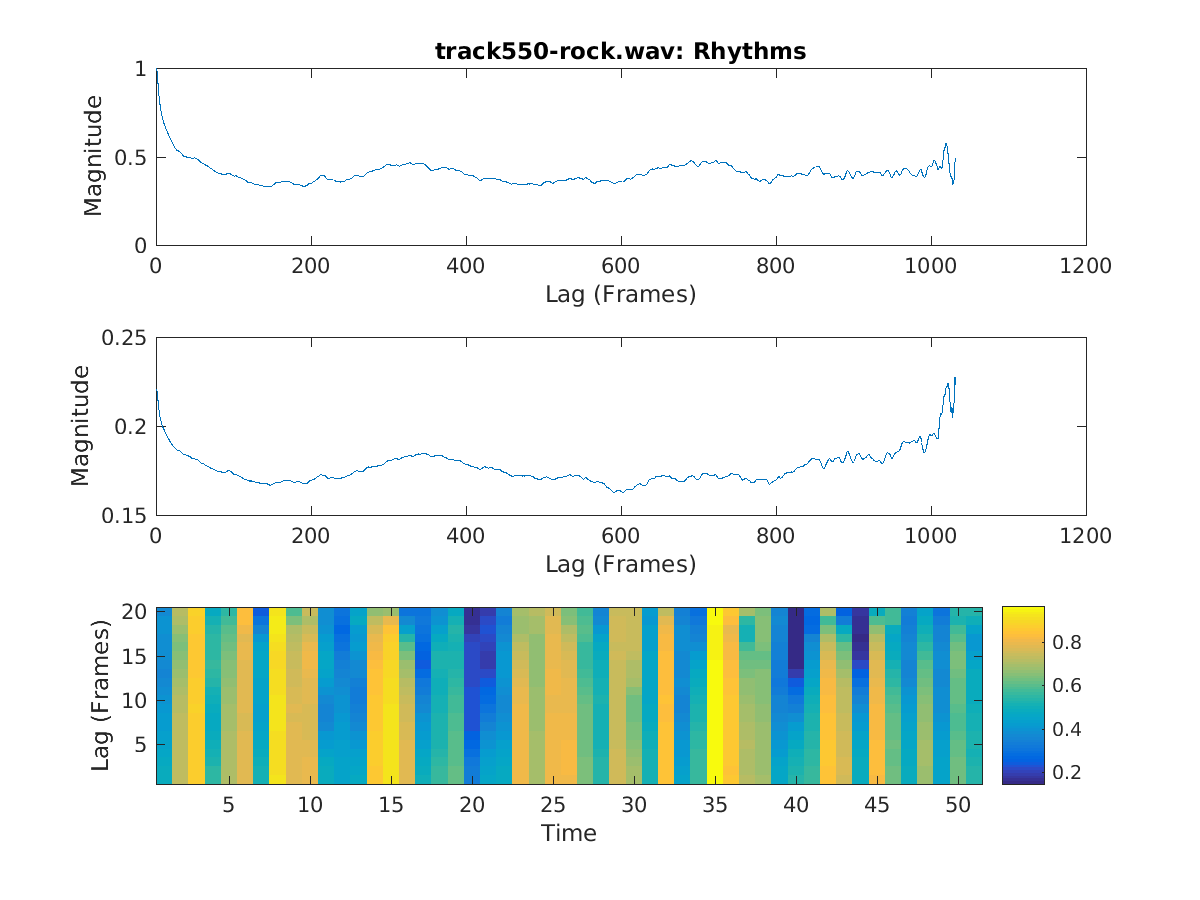
\includegraphics[width=.8\textwidth]{track550-rock-Rhythm.png}
    \caption{track550-rock}
\end{figure}


There are some rhythm artifacts that are seen, that are not as sharp as previous ones. This may be a rhythm over a much larger time frame, but there are no shorter rhythm patterns that can be found. \\

For the variations, the song seems to have different variations, but there are no evidence of a consistent change of rhythm patterns. 


\begin{figure}[H]
    \centering
    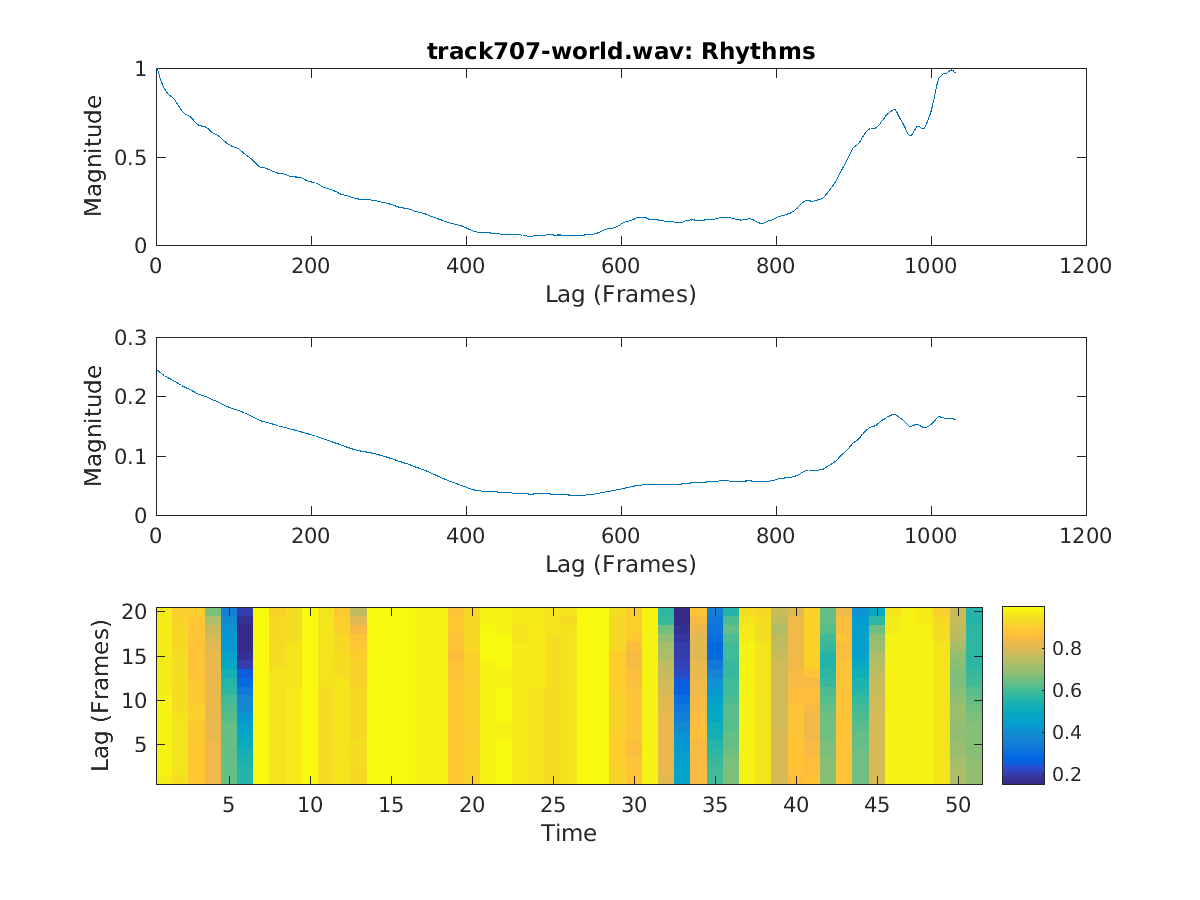
\includegraphics[width=.8\textwidth]{track707-world-Rhythm.png}
    \caption{track707-world}
\end{figure}

There are almost no rhythms found in this track, which makes sense since for most of the frames, there are no changes in the similarity matrices. It takes a sudden dip in both rhythm plots and it does not change a lot. This is clear evidence of no rhythms at all in the song. \\

Looking at the rhythmic variations, there are no variations. It is almost always a large value for the most part when the tone is being played, and this can be seen as well in the mfcc matrix generated in the previous lab. 

\begin{figure}[H]
    \centering
    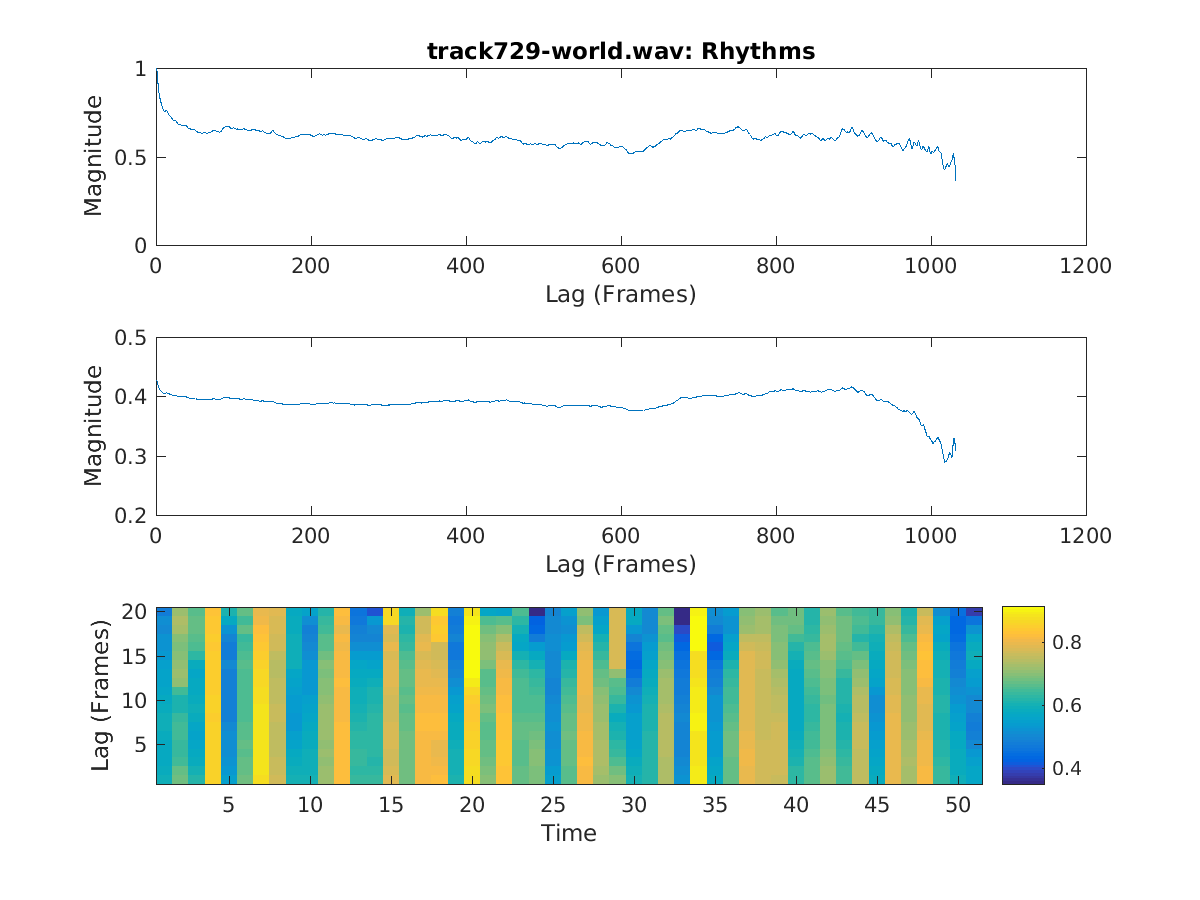
\includegraphics[width=.8\textwidth]{track729-world-Rhythm.png}
    \caption{track729-world}

\end{figure}

There are no obvious rhythm patterns found in either rhythm plots. \\

For the variation, there are slight changes in the rhythm. 


\subsection{Conclusion: Rhythm}

With all three plots, it is very difficult to say whether a song has clear rhythm or not. Although a song may have rhythm, the similarity matrix may find that the other components of a song to be very different, and will not be able to properly classify or catch the rhythm. In addition to classification, rhythm is possible a very bad method of determining genre because it does not capture what defines genre. A rhythm is just a choice musicians make in order to make their music. \\

Overall, it is nice to see the overall patterns songs give, however, it is very difficult to decipher these plots and understand the outputs. 


\section{NPCP}


\lstinputlisting[language=Matlab]{../npcp.m}


Many of the resulting images are hard to comprehend. It is important to keep in mind that the notes that are played are not necessarily aligned with what octave is being played. However, specific notes being used can be noted through the song. \\

In the Y axis, each tick represent the different note being played. The X axis represents time again. The Z axis represents the amplitude of said note. The larger the amplitude, the louder that note is being played. \\

\begin{figure}[H]
    \centering
    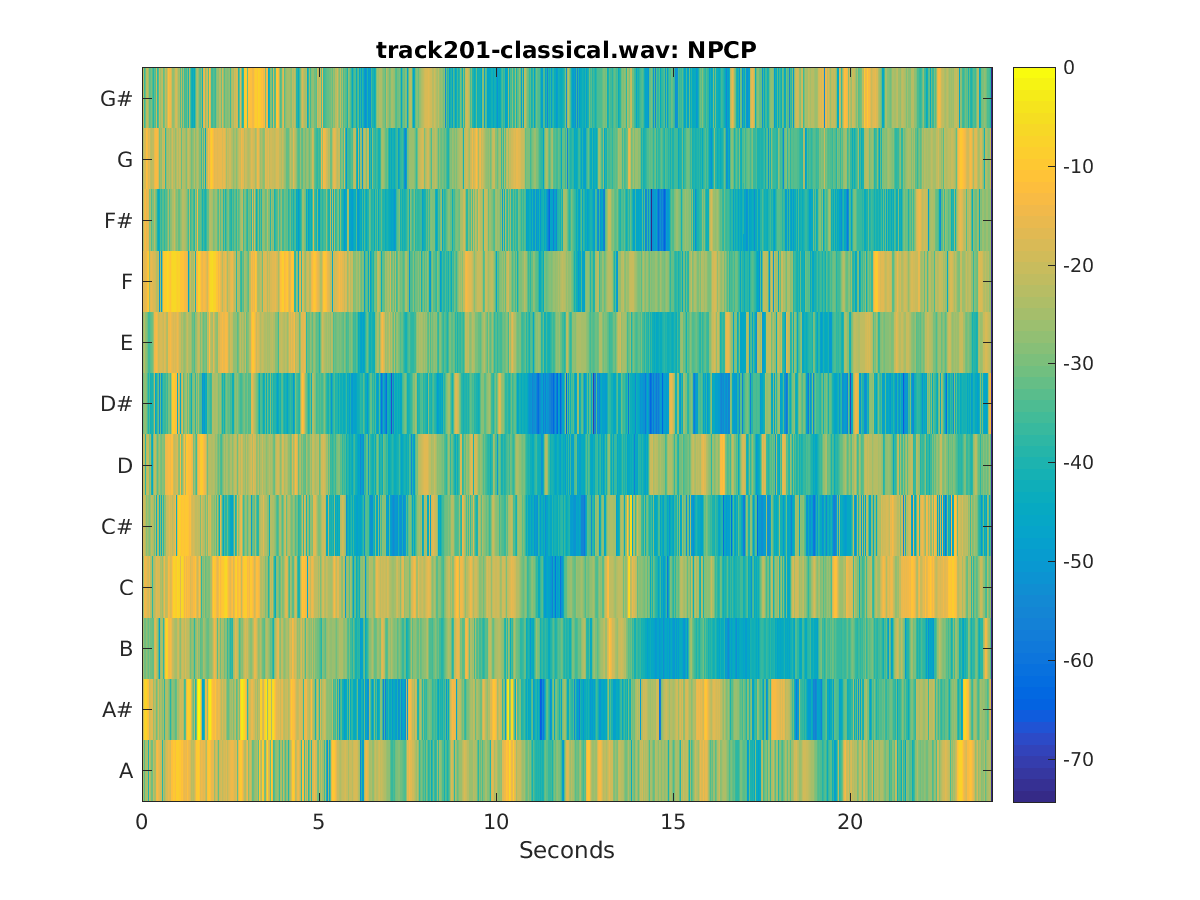
\includegraphics[width=.8\textwidth]{track201-classical-NPCP.png}
    \caption{track201-classical}
\end{figure}


There is not much to say, other than to note the wide variety of notes being used. However, it is key to see that a lot of the sharp notes (A\#, C\#, D\#, F\#, and G\#) are not as commonly used. With classical music, depending on the key being played, this can heavily change what notes are being played. \\


\begin{figure}[H]
    \centering
    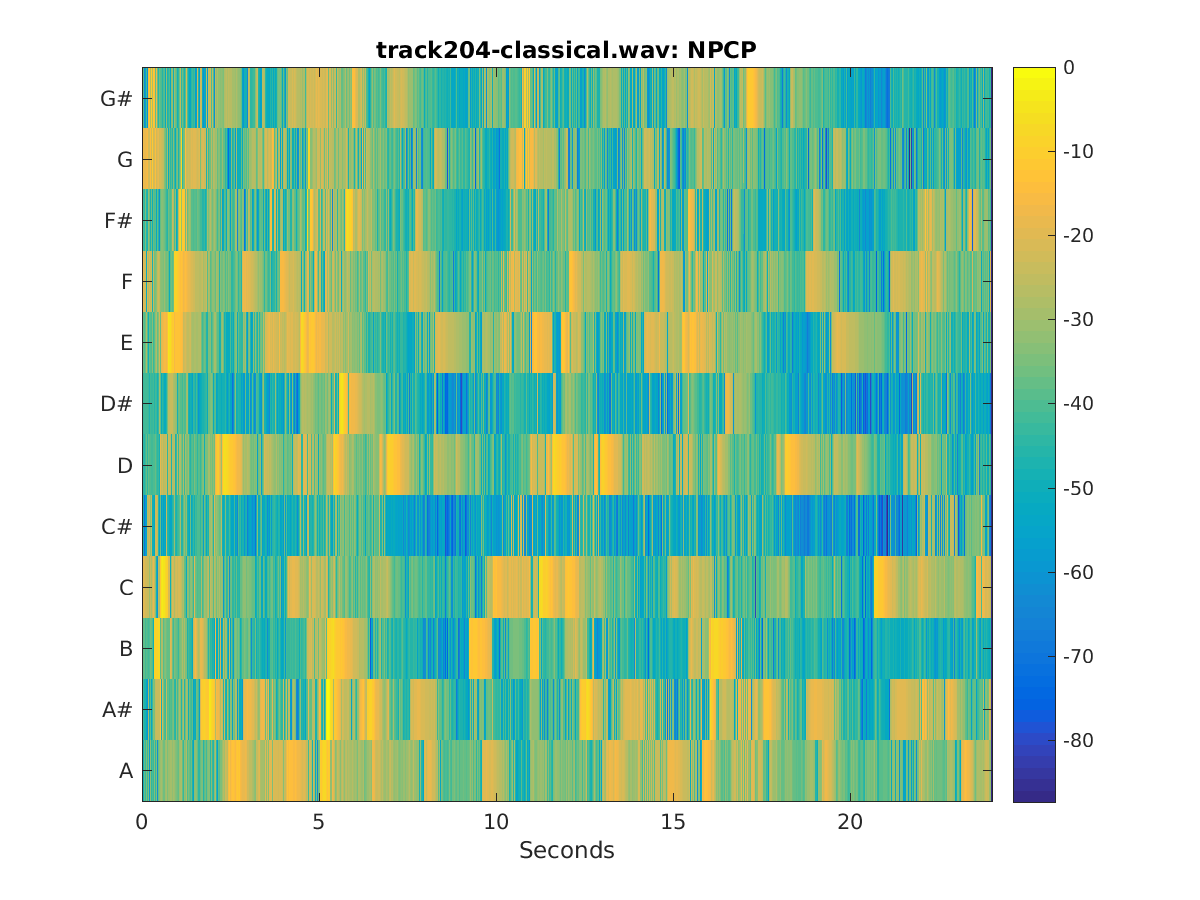
\includegraphics[width=.8\textwidth]{track204-classical-NPCP.png}
    \caption{track204-classical}
\end{figure}

Piano music is beautiful in the fact that you can see the individual notes that are being played over time. This is a key characteristic that can be used to differentiate piano classical music from other genres.\\

\begin{figure}[H]
    \centering
    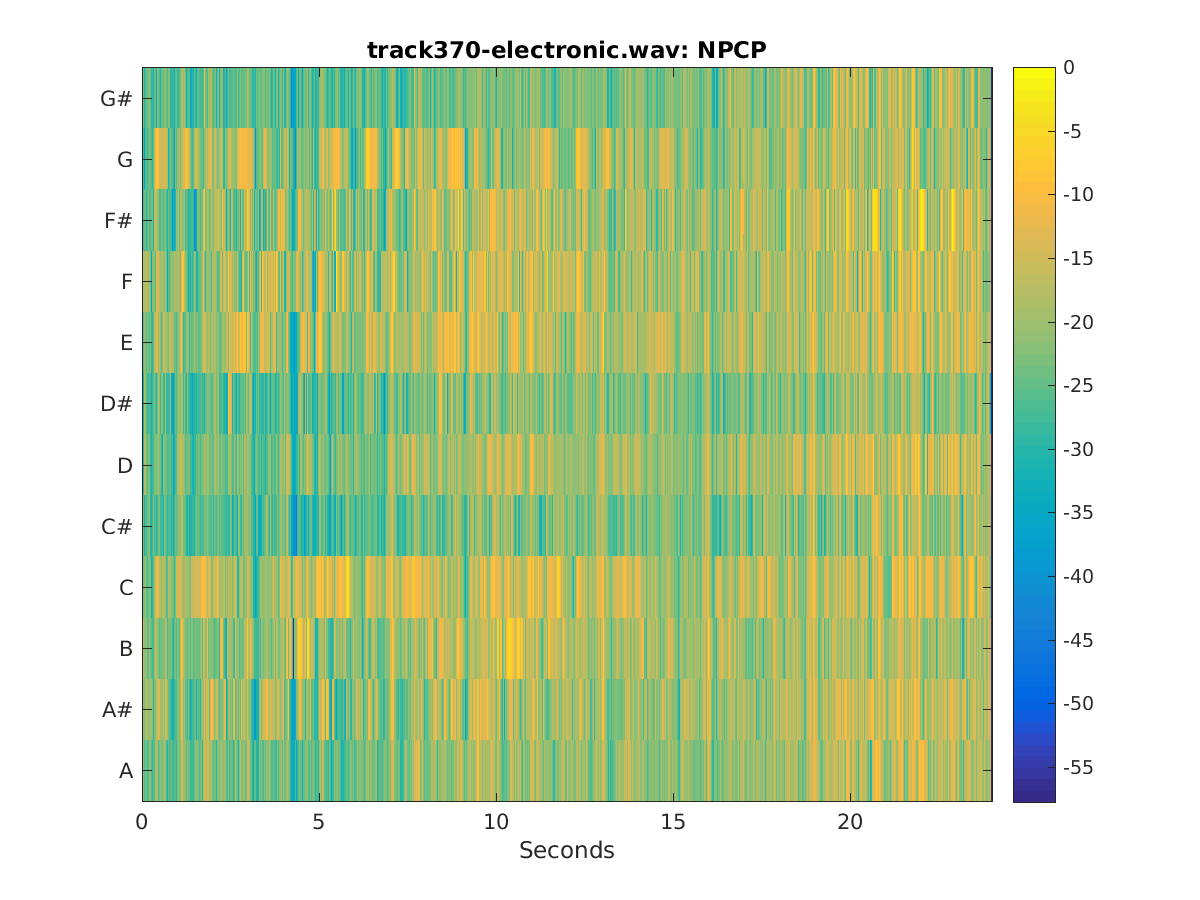
\includegraphics[width=.8\textwidth]{track370-electronic-NPCP.png}
    \caption{track370-electronic}
\end{figure}


Electronic music, unlike classical, is not quite obvious what notes are being played, but more of a wide variety of notes being played back and forth. This pattern may denote a characteristic of the electronic music genre.

\begin{figure}[H]
    \centering
    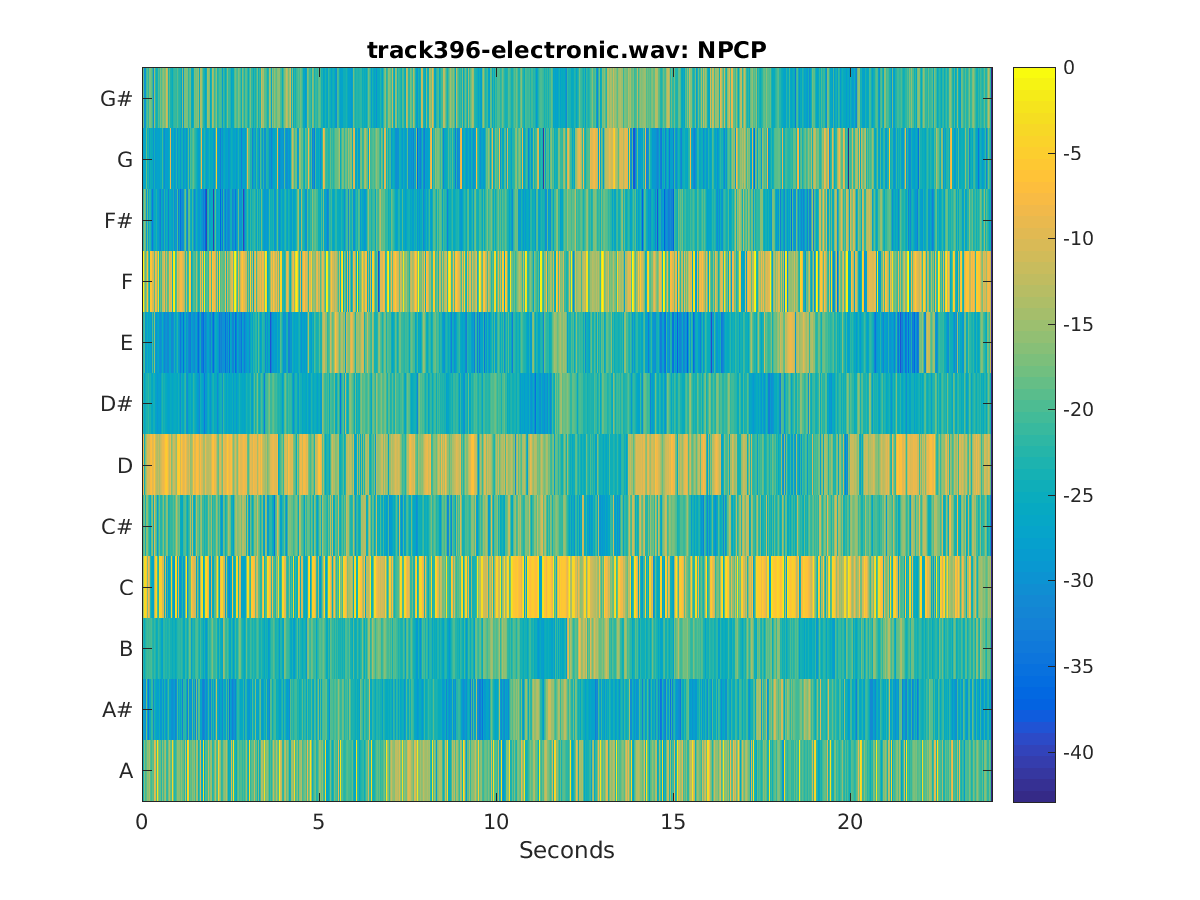
\includegraphics[width=.8\textwidth]{track396-electronic-NPCP.png}
    \caption{track396-electronic}
\end{figure}


Like the previous song, this also shares the same pattern. All the repetitive changes in notes denote a beat pattern used throughout the song. 


\begin{figure}[H]
    \centering
    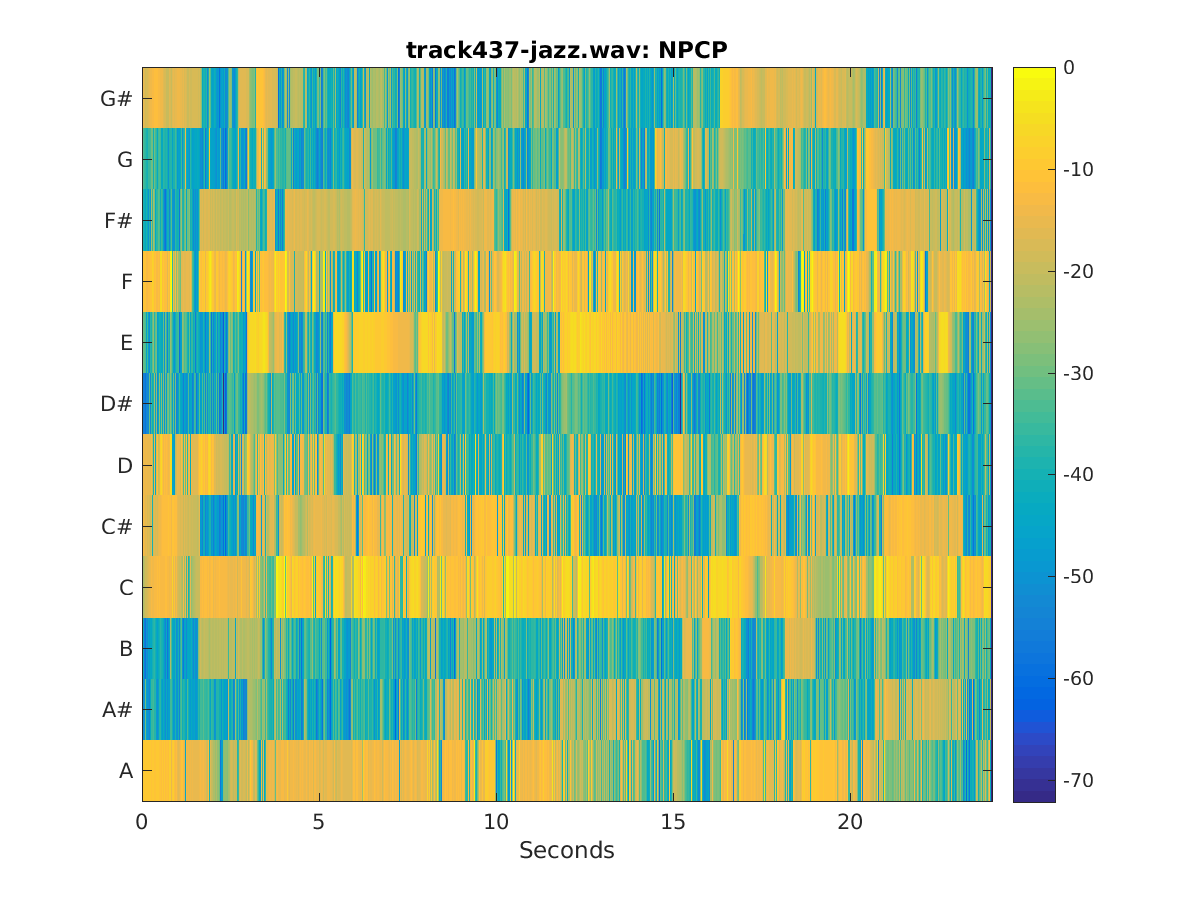
\includegraphics[width=.8\textwidth]{track437-jazz-NPCP.png}
    \caption{track437-jazz}
\end{figure}



Similar to electronic, the notes being played alternate a lot, but there are a few notes that are not as commonly used. This may or may not cause problems when differentiating electronic and jazz.

\begin{figure}[H]
    \centering
    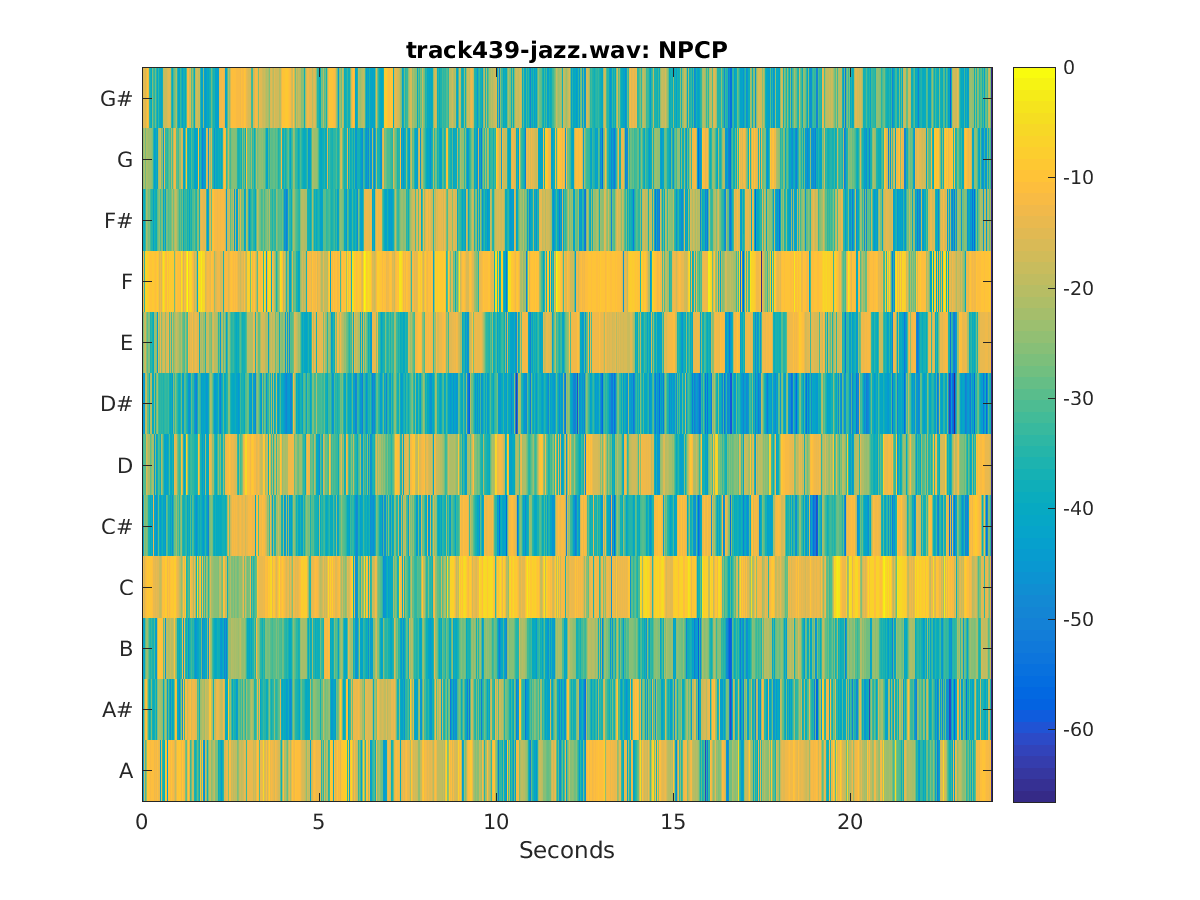
\includegraphics[width=.8\textwidth]{track439-jazz-NPCP.png}
    \caption{track439-jazz}
\end{figure}


The pattern continues as well with this jazz track, but it does also shares common ties with the electronic tracks. The only difference is that there are notes going on and off not as often as electronics.


\begin{figure}[H]
    \centering
    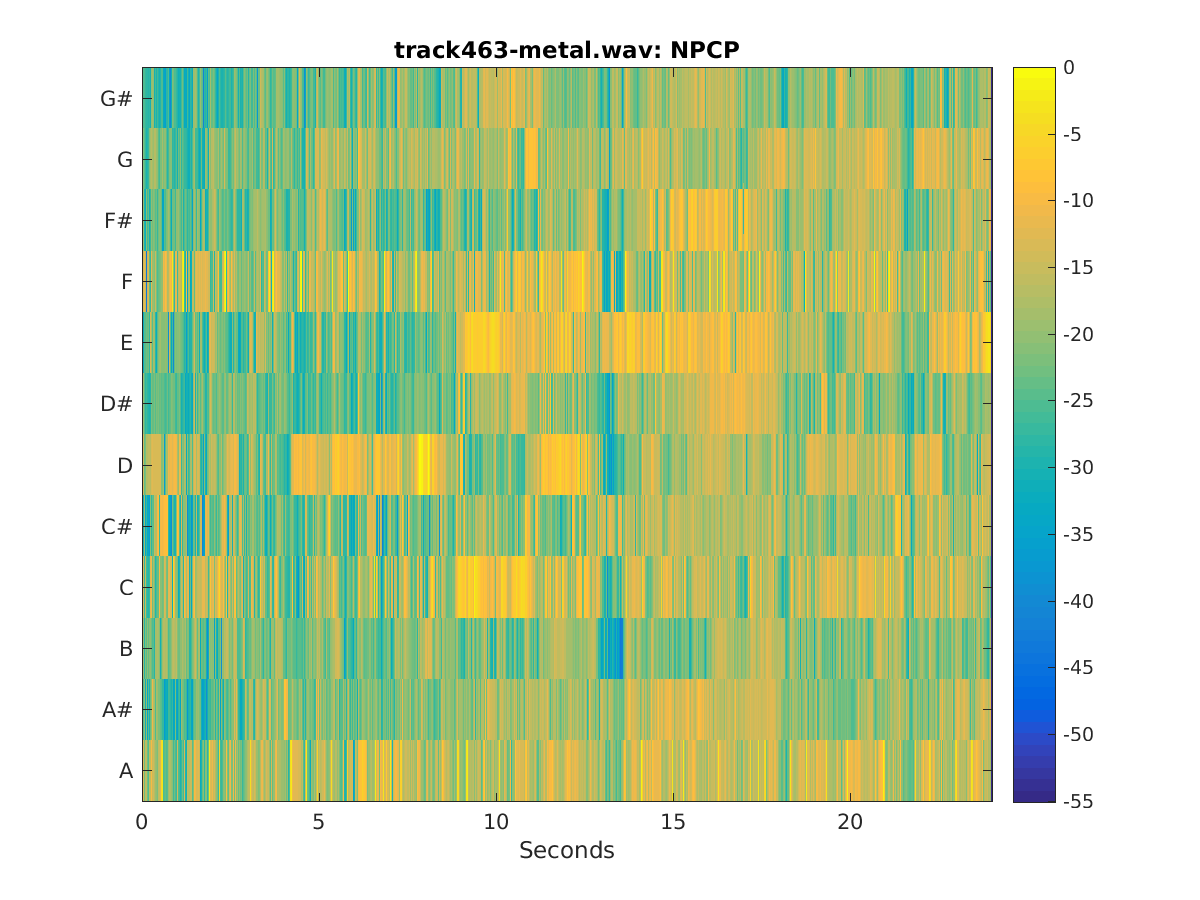
\includegraphics[width=.8\textwidth]{track463-metal-NPCP.png}
    \caption{track463-metal}
\end{figure} 


The metal tracks have a wide variety of notes played. This is significant because unlike the other tracks so far, none have had this type of pattern. Most of the previous songs have had some missing notes, but this metal track covers almost everything.

\begin{figure}[H]
    \centering
    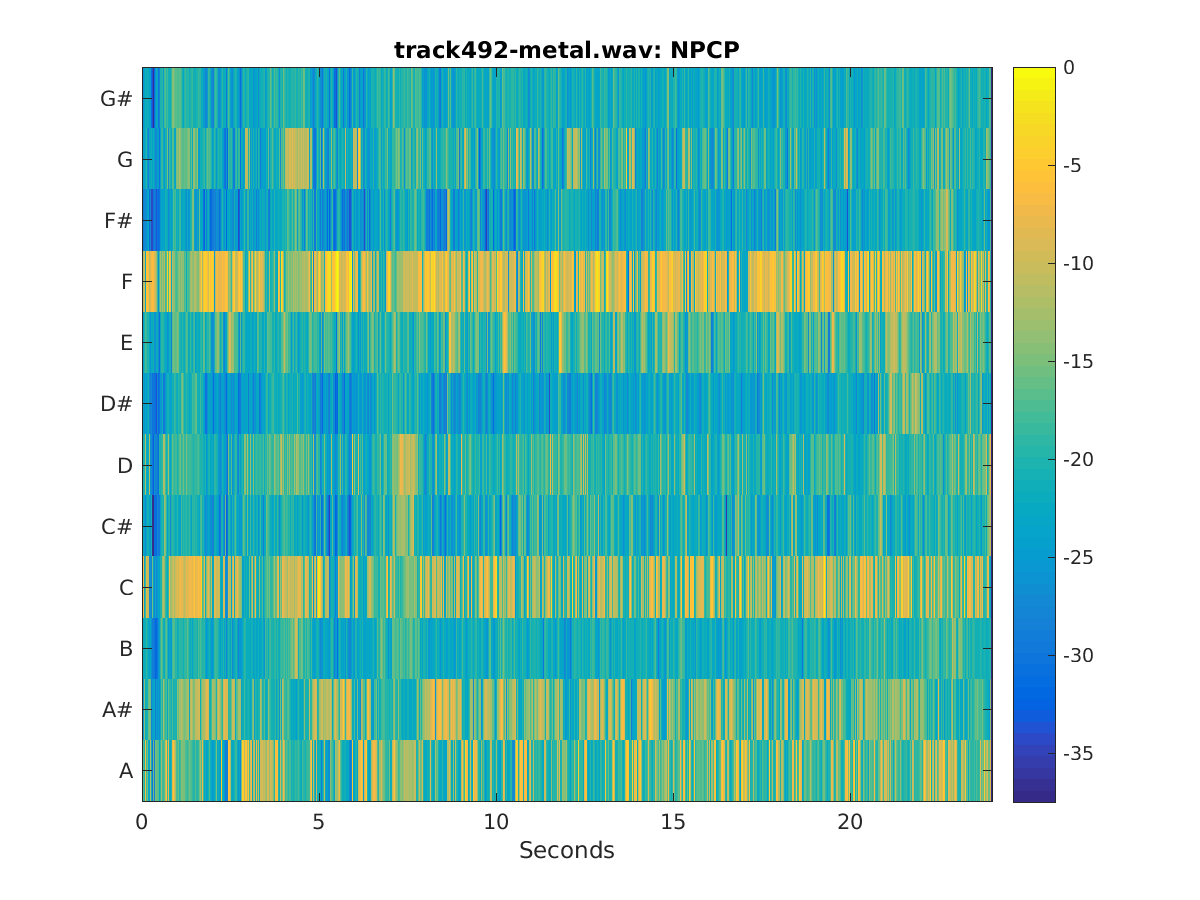
\includegraphics[width=.8\textwidth]{track492-metal-NPCP.png}
    \caption{track492-metal}
\end{figure}


This metal track is very interesting because unlike the previous one, there is only a few selective notes being played. When listening to the track, it becomes very obvious why. There are only two or three instruments playing, and most of them are repeating the same melody.


\begin{figure}[H]
    \centering
    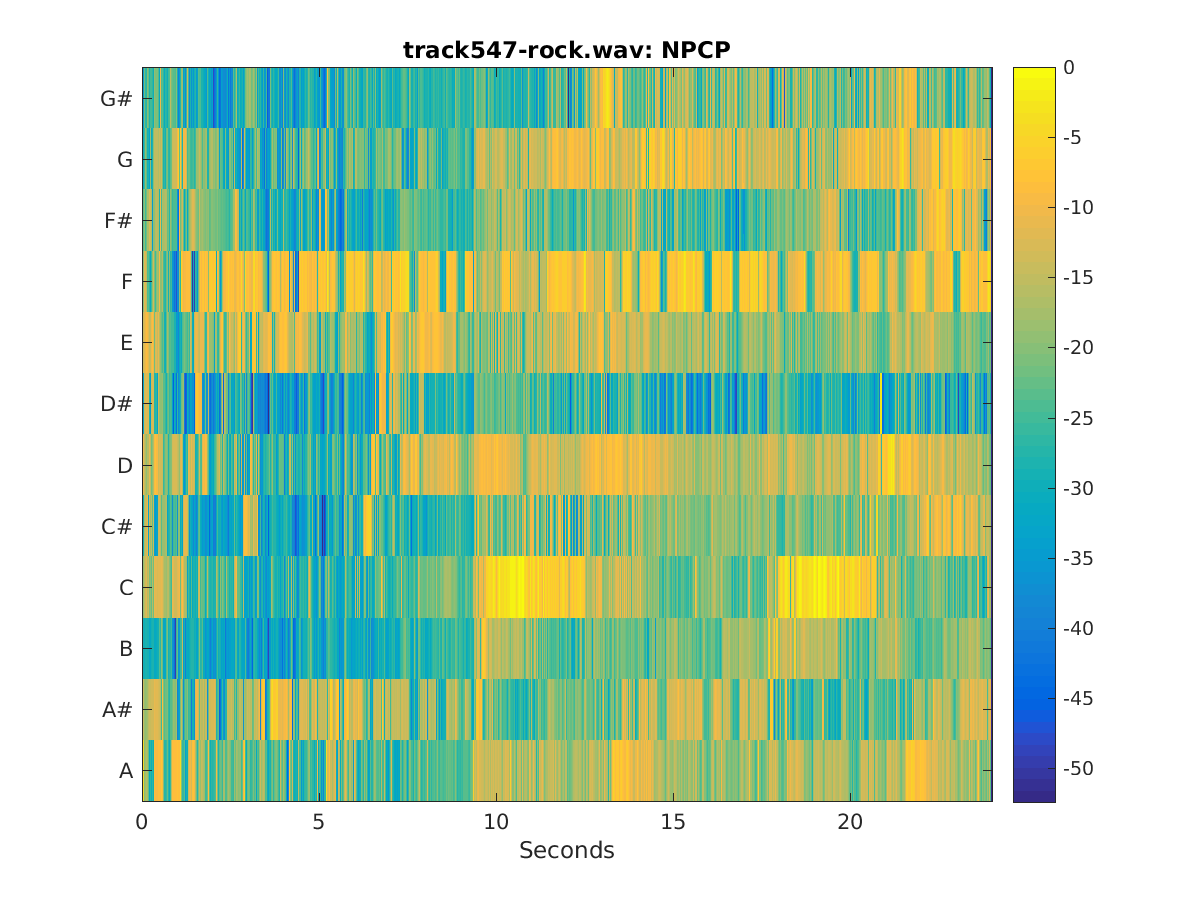
\includegraphics[width=.8\textwidth]{track547-rock-NPCP.png}
    \caption{track547-rock}
\end{figure}


The beginning of the song, there is a melody that is played alone in the beginning that can be seen. At around 10 seconds, other instruments start playing and the increase in other notes are evident. There is a strong increase in the D note.

\begin{figure}[H]
    \centering
    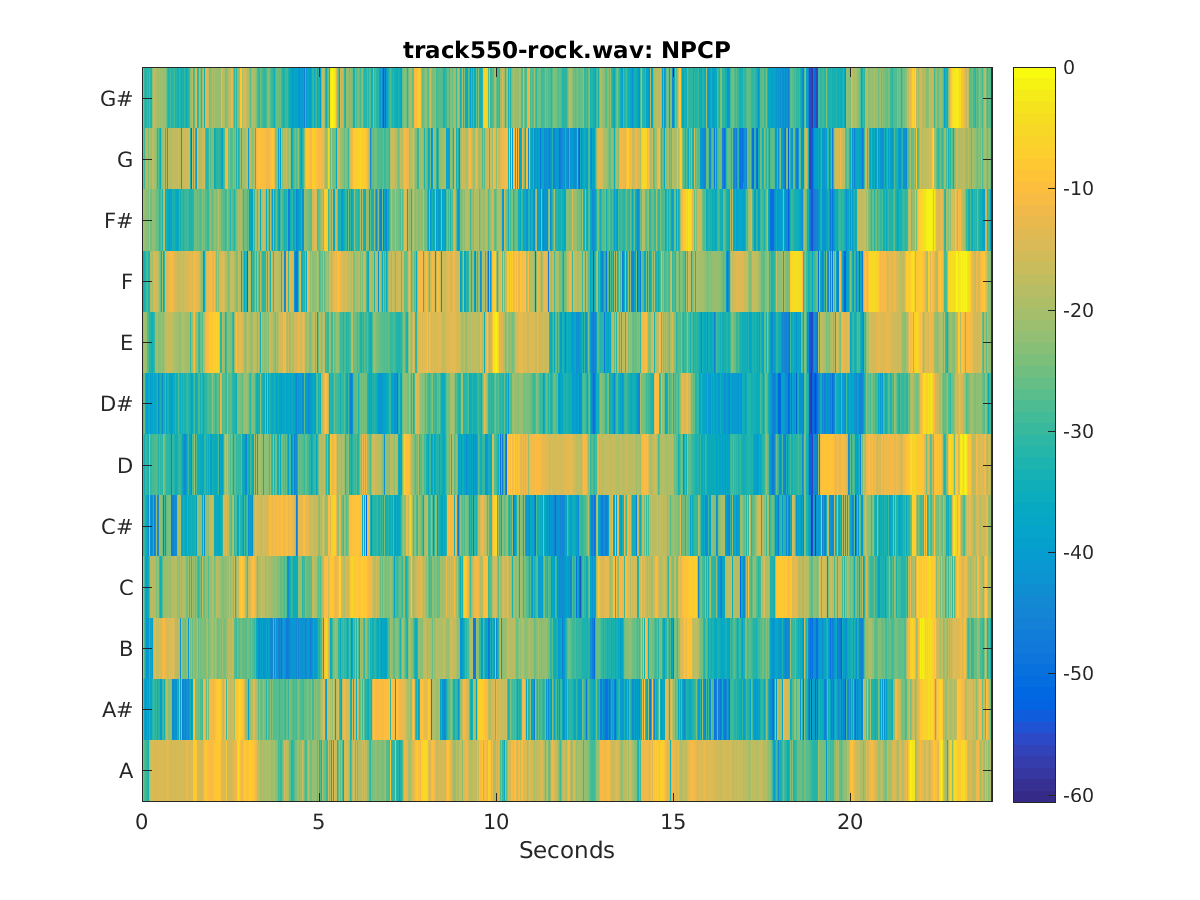
\includegraphics[width=.8\textwidth]{track550-rock-NPCP.png}
    \caption{track550-rock}
\end{figure}


The last rock track shares certain patterns, such as a single note being stronger than the other notes. The other key factor that two songs share is the fact that there are lots of notes that are not being used. 

\begin{figure}[H]
    \centering
    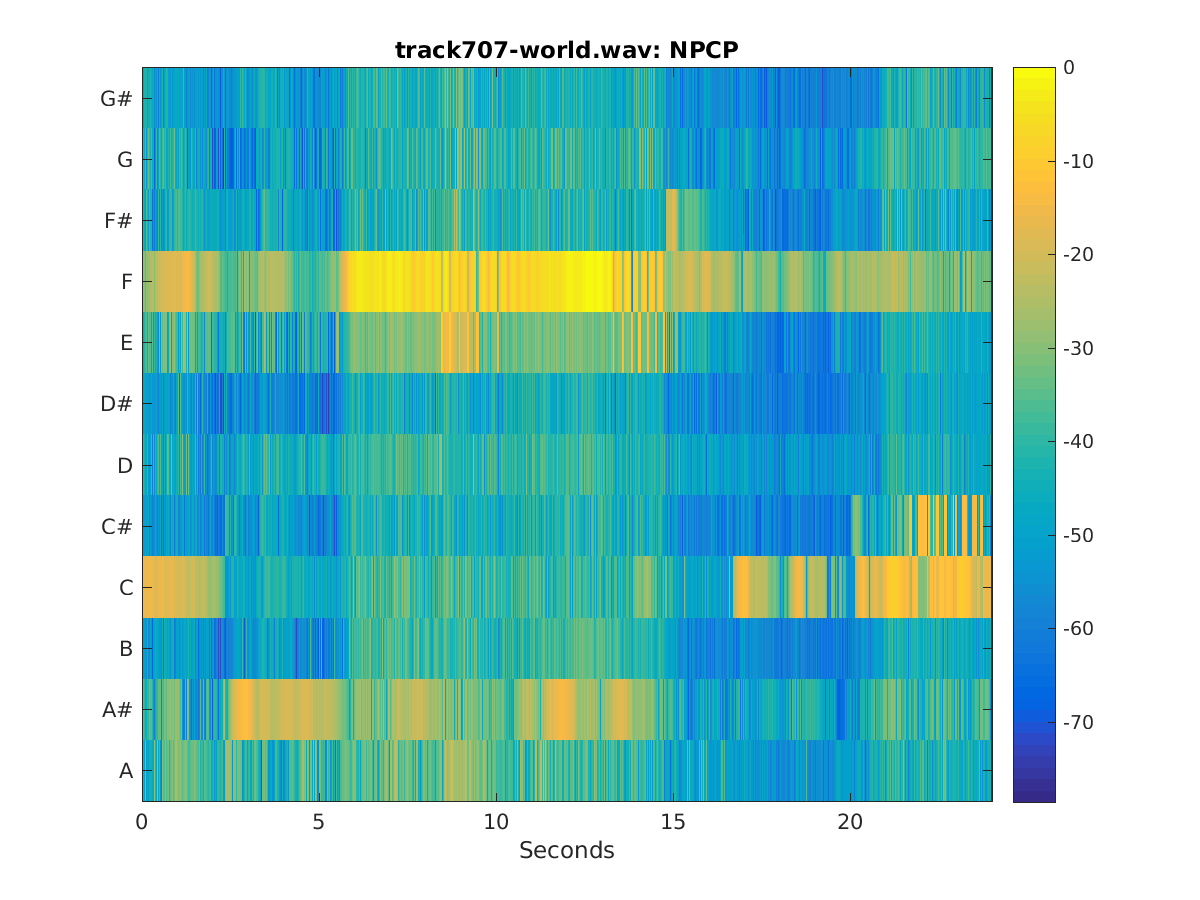
\includegraphics[width=.8\textwidth]{track707-world-NPCP.png}
    \caption{track707-world}
\end{figure}

There are obviously a few notes being played by the same instrument. This is very similar to the piano track, where individual notes being played are obvious, but there are slight differences as some parts of the song has lots of other frequencies.
\begin{figure}[H]
    \centering
    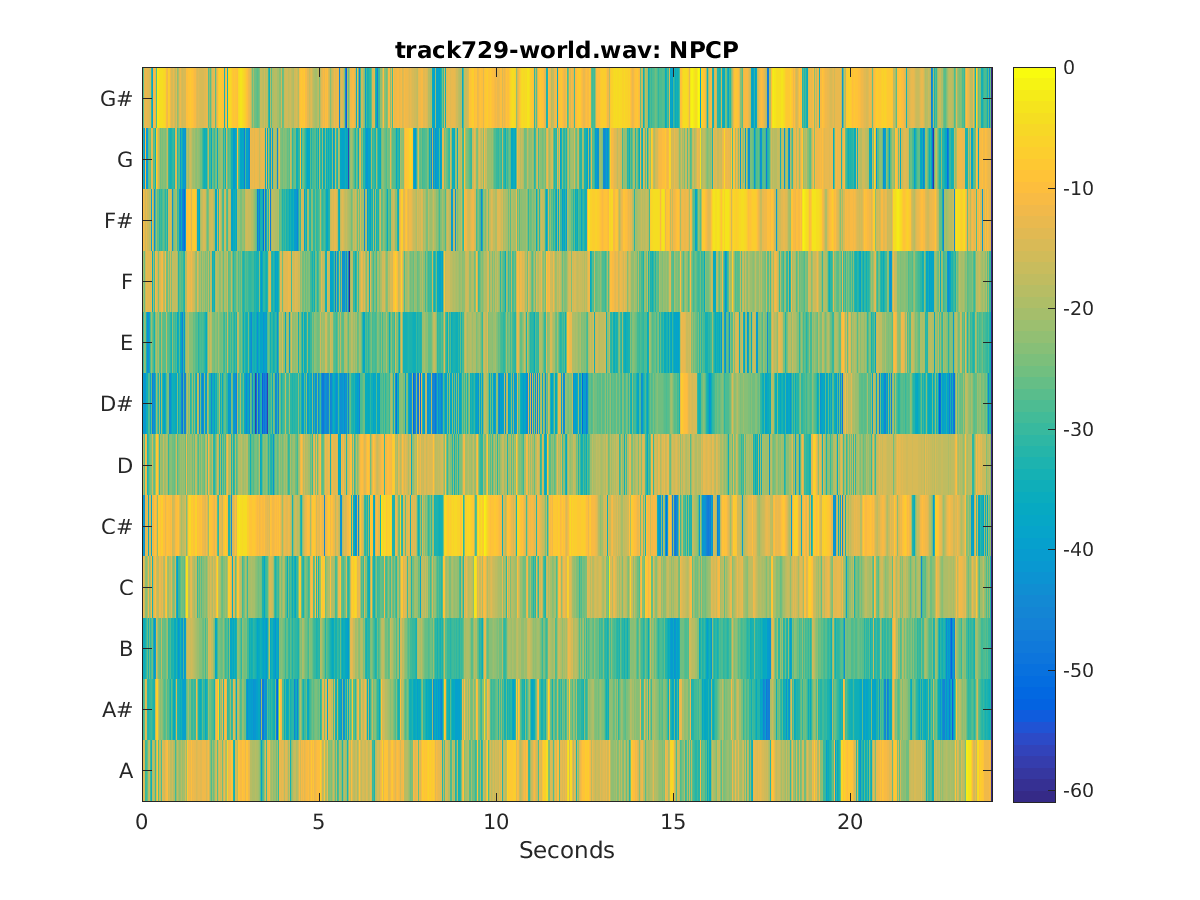
\includegraphics[width=.8\textwidth]{track729-world-NPCP.png}
    \caption{track729-world}
\end{figure}

The last world track shares some characteristics of the previous one. It has very specific note ranges it plays in. 

\subsection{Conclusion: NPCP}

The chroma analysis demonstrates a powerful tool that allows us to see the actual differences between the audio tracks, however, this alone might not be able to differentiate the different genres.

\appendix

\section{Code}

\subsection{Workspace Script}
\lstinputlisting[language=Matlab]{../workspace.m}

\subsection{Save Image Function}
\lstinputlisting[language=Matlab]{../saveImage.m}

\end{document}
